\documentclass{article}


% if you need to pass options to natbib, use, e.g.:
%     \PassOptionsToPackage{numbers, compress}{natbib}
% before loading neurips_2023


% ready for submission
\usepackage{neurips_2024}


% to compile a preprint version, e.g., for submission to arXiv, add add the
% [preprint] option:
%     \usepackage[preprint]{neurips_2023}


% to compile a camera-ready version, add the [final] option, e.g.:
%     \usepackage[final]{neurips_2023}


% to avoid loading the natbib package, add option nonatbib:
%    \usepackage[nonatbib]{neurips_2023}


\usepackage[utf8]{inputenc} % allow utf-8 input
\usepackage[T1]{fontenc}    % use 8-bit T1 fonts
\usepackage[hidelinks]{hyperref}       % hyperlinks
\usepackage{url}            % simple URL typesetting
\usepackage{booktabs}       % professional-quality tables
\usepackage{amsfonts}       % blackboard math symbols
\usepackage{nicefrac}       % compact symbols for 1/2, etc.
\usepackage{microtype}      % microtypography
\usepackage{xcolor}         % colors
\usepackage{multirow}
\usepackage{xspace}

\usepackage{longtable}
\usepackage{multirow}
\usepackage{graphicx}
\usepackage{lineno}
\usepackage{siunitx}
\usepackage{float}
\usepackage{array}
\usepackage{amsmath}
\usepackage{subcaption}
\usepackage{enumitem}
\usepackage{xcolor}
\usepackage{xspace}
\usepackage{booktabs}
\usepackage{tabularx}
\usepackage[utf8]{inputenc}
\usepackage{geometry}
\usepackage{tcolorbox}
\linenumbers

%%%%%%%%%%%%%%%%%%%%%%%%%%%%%%%%%%%%%%%%%%%%%%%%%%%%%%%%%%%%%%%%%%%%%%%%%%%%%%%%%%%%%%
% Add all custom commands here

\newcommand*\samethanks[1][\value{footnote}]{\footnotemark[#1]}
 \newcommand{\kc}[1]{\textcolor{red}{Kartik: #1}}
%\newcommand{\kc}[1]{}
\newcommand{\dieuwke}[1]{\textcolor{red!50!blue!80}{DH: #1}}
% \newcommand{\dieuwke}[1]{}

% Custom font for evaluation and judge model names
\definecolor{darkgreen}{RGB}{0,100,0}
\definecolor{red}{RGB}{255,0,0}
% \newcommand{\eval}[1]{{\textcolor{darkgreen}{#1}}}
\newcommand{\eval}[1]{{\fontfamily{phv}\selectfont #1}}
\newcommand{\judge}[1]{\texttt{\textcolor{black}{#1}}}

\newcommand{\njudges}{9\xspace}
\newcommand{\nexamtakers}{9\xspace}

\newcommand{\evaluatormodel}{exam-taker model\xspace}
\newcommand{\evaluatormodels}{exam-taker models\xspace}
\newcommand{\Evaluatormodel}{Exam-taker model\xspace}
\newcommand{\Evaluatormodels}{Exam-taker models\xspace}

\newcommand{\judgemodel}{judge model\xspace}
\newcommand{\judgemodels}{judge models\xspace}
\newcommand{\Judgemodel}{Judge model\xspace}
\newcommand{\JudgeModel}{Judge Model\xspace}
\newcommand{\Judgemodels}{Judge models\xspace}
\newcommand{\JudgeModels}{Judge Models\xspace}

\newcommand{\specialcell}[2][c]{\footnotesize\begin{tabular}[#1]{@{}l@{}}#2\end{tabular}}

% \def\mytcolorbox#1#2#3{
% \begin{tcolorbox}[outerbox, title={\textit{#1}}]
%   \begin{tcolorbox}[colback=lightorange, colframe=myorange!75!black, boxrule=0.5mm, sharp corners, rounded corners]
%     \texttt{#2}
%   \end{tcolorbox}
%   \vspace{1em}
%   \texttt{#3}
% \end{tcolorbox}
% }

\def\mytcolorbox#1#2#3{
\begin{tcolorbox}[outerbox, title={\textit{#1}}]
\texttt{#2} \\
\\
\texttt{#3}
\end{tcolorbox}
}
%%%%%%%%%%%%%%%%%%%%%%%%%%%%%%%%%%%%%%%%%%%%%%%%%%%%%%
% Cleverref
\usepackage[noabbrev,capitalize,nameinlink]{cleveref}
\crefname{section}{Section}{Sections}%{\S}{\S\S}
\crefname{table}{Table}{}
\crefname{figure}{Figure}{}
\crefname{section}{\S}{\S\S}
\Crefname{section}{\S}{\S\S}
\crefname{appendix}{Appendix}{Appendices}
\Crefname{Appendix}{Appendix}{}

%%%%%%%%%%%%%%%%%%%%%%%%%%%%%%%%%%%%%%%%%%%%%%%%%%%%%%%%%%%%%%%%%%%%%%%%%%%%%%%%%%%%%%
\title{Judging the Judges: Evaluating Alignment and Vulnerabilities in Judge LLMs}


% The \author macro works with any number of authors. There are two commands
% used to separate the names and addresses of multiple authors: \And and \AND.
%
% Using \And between authors leaves it to LaTeX to determine where to break the
% lines. Using \AND forces a line break at that point. So, if LaTeX puts 3 of 4
% authors names on the first line, and the last on the second line, try using
% \AND instead of \And before the third author name.


\author{%
  Aman Singh Thakur\thanks{Equal contribution}\\
  College of Information \& Computer Sciences\\
  University of Massachusetts\\
  \texttt{amansinghtha@umass.edu} \\
  \And
  Kartik Choudhary\samethanks\\
  College of Information \& Computer Sciences\\
  University of Massachusetts\\
  \texttt{kartikchoudh@umass.edu} \\
  \And
  Venkat Srinik Ramayapally\samethanks\\
  College of Information \& Computer Sciences\\
  University of Massachusetts\\
  \texttt{vramayapally@umass.edu} \\
  \And
  Sankaran Vaidyanathan\\
  College of Information \& Computer Sciences\\
  University of Massachusetts\\
  \texttt{sankaranv@cs.umass.edu} \\
  \And
  Dieuwke Hupkes\\
  % Fundamental AI Research (FAIR) Lab\\
  Meta\\
  \texttt{dieuwkehupkes@meta.com} \\
}




\begin{document}

\hyphenpenalty=10000
\maketitle

\begin{abstract}
The \textit{LLM-as-a-judge} paradigm is rapidly gaining traction as an approach to evaluating Large Language Models (LLMs), as it offers a promising solution to the scalability challenges associated with human evaluation. 
However, relatively little is known about the strengths, weaknesses, and potential biases associated with this setup.
% While previous studies primarily focus on LLMs' capacity as human proxies, there's a crucial need to gauge their effectiveness against humans in simple, objective scenarios first. 
In this paper, we present a comprehensive study involving various pairs of LLMs -- both base and instruction-tuned models -- evaluated alongside human annotations. 
Leveraging TriviaQA as a benchmark for assessing objective knowledge reasoning, we conduct a comprehensive study of the performance of various LLMs acting as judges, as well as their alignment with human judgments across different sizes, families, few-shot scenarios, and judge prompts. 
Our research uncovers substantial misalignment between \judgemodels and human annotations, and we show that even when they exhibit significant alignment, this does not necessarily translate to similar evaluation scores. 
We conduct an exhaustive error analysis, highlighting vulnerabilities inherent in Judge LLMs, particularly in instruction-tuned models. 
Additionally, we explore prompt sensitivities and biases in \judgemodels and propose potential strategies for improving their accuracy. 
\end{abstract}


\section {Introduction} \label{sec:intro}


Over the last few years, Large Language models (LLMs) have been shown to possess remarkable world knowledge \citep{petroni2019language, razeghi2022impact} and the ability to learn specialized tasks from a few examples \citep{brown2020language}. 
LLMs have been employed in various tasks including generating free-form responses, condensing extensive textual data, conducting searches, categorizing or grouping documents, and facilitating question-answering systems \citep{vectara_llm_use_cases}. 
As more and more new LLMs with different architectures and training methods continue to be released, there is a need for tools that can accurately evaluate their capabilities and limitations across a variety of tasks. 

However, the empirical evaluation of LLMs has so far shown to be a challenging and non-trivial task, primarily due to the diversity of output they generate and the wide range of tasks they are used for \citep{Zhang2024LLMEval, li2023generative}. 
Various methods have been proposed for evaluating LLMs, typically falling into one of two broad categories. 
Benchmarks such as MMLU \citep{mmlu}, TruthfulQA \citep{lin2021truthfulqa}, and GSM8K \citep{cobbe2021training} are used to evaluate specific capabilities of LLMs in an automated manner. 
Additionally, leaderboards like Chatbot Arena \citep{chiang2024chatbot} and Open LLM Leaderboard \citep{open-llm-leaderboard} assign ranks to models considering pair-wise rankings of LLM outputs, done by humans or, in some cases, automated evaluation methods.

Since both strategies involve evaluating free-form text responses generated by the LLMs, evaluating the responses is often just as challenging as generating them in the first place \citep[see e.g.][]{chang2023survey}. 

%One solution to this problem is to formulate benchmarks as multiple-choice questions (MCQ), and compare the log-probabilities of the potential answers rather than evaluating the generated answer directly. 
%However, the MCQ paradigm severely limits the range of abilities that can be evaluated, and this setup increasingly diverges from how LLMs are used in practice.

The use of lexical matching methods such as exact match (EM) or n-gram overlap to evaluate the responses are practical and cost-efficient approaches, but are susceptible to false negatives and often fail to adequately distinguish between responses with subtle differences that change their semantic meaning.
%
This issue is exacerbated when evaluating instruction-tuned ``chat'' models that are fine-tuned to carry out conversations with humans in natural language, since their responses tend to be more verbose \citep{saito2023verbosity, renze2024benefits}. 

\kc{Should this paragraph go in Related Work?}
For these reasons, human evaluation remains the gold standard for evaluating LLM responses. %, especially since many benchmarks aim to assess how useful the LLMs are to humans. 
However, human evaluation is expensive, time-consuming, and often impractical in many use cases. 
As a result, it has increasingly become common practice to evaluate LLM responses using another LLM as a \judgemodel \citep[e.g.][]{lin2021truthfulqa,islam2023financebench,chiang2023can,liusie2024llm}.
Prior work has demonstrated that LLMs such as \judge{GPT-4} exhibit high alignment with humans in such tasks when used as a judge \citep{sottana2023evaluation,zheng2024judging}. 
Despite promising results in various settings, \judgemodels still suffer from the issues of current LLMs, such as hallucinations and factual errors \citep{ye2023cognitive, turpin2023language} and difficulty in following complex instructions \citep{li2023instruction, he2024can}. Moreover, use of LLMs as judges can give rise to unique challenges such as exhibiting position bias \citep{pezeshkpour2023large} and verbosity bias \citep{saito2023verbosity} in their preference, confusing the evaluation criteria \citep{hu2024llm}, or focusing more on the style and grammar of the response compared to its factuality \citep{wu2023style}.
% However, the strengths, weaknesses and biases of this \emph{LLM-as-a-judge} paradigm have not been studied in detail.
%
% As much of the contemporary research in LLMs and vision-language models is guided by empirical results, it is important to ensure that the results of various benchmarks for LLMs reflect the true capabilities of the models and are not artifacts of the various choices surrounding the benchmarks and their evaluations.

In this work, we assess the accuracy of LLMs as judges and investigate their properties, comparing them with human evaluation and automated evaluation methods. 
\textbf{The primary contribution of this work is an extensive study of how well various popular LLMs perform when acting as judges, along with an analysis of how their performance varies across different \judgemodels and evaluation strategies}. 
While previous studies on the accuracy of LLMs as judges have relied on measuring the alignment of LLM judgments with human judgments, we find that LLMs with similar human alignment can differ significantly on the questions they evaluate incorrectly. 
\textbf{The second contribution of this work is an investigation of the ``characters and styles'' of different LLMs as judges, and their susceptibility to different kinds of errors}.

% Key results: There is variation in scores given by judges, even ones with high alignment. There is pre-trained to instruction-tuned unlearning happening, but not to the degree suggested by EM.

\section {Related Work}\label{sec:relatedwork}

LLMs have been used as judges to evaluate performance of other LLMs on various tasks, including evaluation of story generation \citep{chiang2023can}, retrieval-augmented generation \citep{es2023ragas},  visual QA \citep{maas2024improving}, as well as code comprehension \citep{yuan2023evaluating} and multilingual evaluation \citep{hada2023large}. \citet{Zhang2024LLMEval} and \citet{sottana2023evaluation} have proposed ways to standardize LLM evaluations, and the roles the \judgemodels might play in such solutions.
%
Position bias has been observed in many setups using LLMs as judges \citep{zheng2023large, wang2023large}, and methods like alignment-based calibration systems \citep{li2023split} and permutation self-consistency \citep{tang2023found} have been proposed as possible mitigations.

\citet{judgingllms} study the alignment of \judgemodels with humans on open-ended tasks. \citet{selfrewardingmodels} use LLMs as evaluators to construct self-rewarding models, which are subsequently employed for training and fine-tuning other LLMs.
%
\citet{liusie2024llm} have shown that LLMs perform better in comparative assessment compared to absolute scoring, which can be used for reliably measuring the relative performance of models \citep{liu2024aligning} and creating classifiers for pairwise grading \cite{llmasclassifier}.
%
\citet{zeng2023evaluating} have proposed a benchmark for evaluating the performance of LLMs as judges. \citet{shankar2024validates} introduce an iterative method for aligning \judgemodels to humans by generating evaluation criteria and assertions. \citet{judgelm} have proposed fine-tuning LLMs to improve their performance as judges.

% While there exist leaderboards for assessing automatic evaluation of instruction-following models such as \citet{alpaca_eval} and \citet{evaluationinsttunedbench}, there is a dearth of research exploring the viability of employing LLMs as judges for Core Knowledge Benchmarks. Notably, \citet{openqa} conducted a study on core knowledge benchmarks like TriviaQA \cite{triviaqa} and Natural Questions \cite{naturalquestions}, but failed to encompass the entire spectrum of LLMs available for examination.

% Several frameworks have been proposed to delve deeper into LLM evaluation \cite{li2023beyond}, and to utilize judge models as . 
% \section{Background} \label{sec:background}

% \textcolor{red}{TODO}

\section{Methodology} 
\label{sec:methodology}

% \kc{Describe metrics and how to perform  benchmarks here so that in the next section we talk about what specific experiments we are running? Right now they are kind of mixed I think.}

We evaluate the strengths and weaknesses of the LLM-as-a-judge paradigm by focusing on the relatively straight-forward assessment task of judging answers to the questions of a knowledge-reasoning benchmark.
We consider \njudges \judgemodels, that assess the responses of \nexamtakers \evaluatormodels. 
%
The benchmark questions are provided to the \evaluatormodels and their responses are recorded to be evaluated by the \judgemodels.
%

% \section{Experiments}

% Results of a benchmark, as evaluated by the judge, can be used in different ways – establishing a
% relative ordering of LLMs based on their performance [cite], creating a quantitative measure of their
% capabilities in a particular domain [cite], developing/distilling other LLMs, etc. The metrics used to77
% gauge the quality of the evaluations from a judge, therefore, depend on the final use-cases for the
% benchmark results and the reliability of the benchmark results.
% To understand the strengths and weaknesses of different judges, we benchmark pre-trained and80
% instruction-tuned evaluation models across a wide variety of model sizes, and examine the quality
% of the evaluations from different judge models. Specifically, we conduct experiments to answer the
% following research questions: 1) How well do the evaluations from different judges align with human
% evaluations? 2) How is a alignment of evaluations related to the alignment of the final scores given
% by the judges? 3) How similar are the rankings of evaluation models generated by the judge models
% compared to the rankings by humans? 4) How sensitive are the judge models to the specific prompt
% provided to them to give a judgement? 5) What are the similarities and differences in the mistakes
% made by different judges?

\subsection{Benchmark and evaluation metrics} 
\label{sec:experiments:benchmark}
We use the TriviaQA  dataset\citep{joshi2017triviaqa} consisting of 95K question-answer pairs sourced from 14 trivia and quiz league websites. 
%
Each question in the train and validation set is annotated with alist of short answers containing a minimal set of facts and evidence documents collected from Wikipedia and the Web.
The benchmark is done on the validation set and short answers are used as references for the judges while grading. 
The training and validation sets both come from the \texttt{unfiltered} partition of the dataset.
%
To stay closer to the typical scenarios in which LLMs may be used as judges, we focus on questions with ten or fewer reference answers.

For the experiments that require manual annotation of the \evaluatormodel responses, the benchmarks are done on a random sample of $400$ questions from the dataset.
%
For other experiments that do not require human annotation, the entire validation set is used for the benchmarks.
%
We primarily use score, alignment, and Cohen's kappa coefficient to evaluate judges. The definitions of each of the metrics is explained in detail in \cref{app:metrics}
%  

\subsection{\Evaluatormodels} \label{sec:experiments:evaluationmodel}
To understand the strengths and weaknesses of different judges, we benchmark pre-trained (base) and instruction-tuned (chat) \evaluatormodels across a wide variety of model sizes, and examine the quality of the evaluations from different \judgemodels.
In particular, we consider \eval{Llama-2} in 7B, 13B, and 70B parameter sizes for both base and chat versions \citep{touvron2023llama}, \eval{Mistral 7B} in base and chat versions \citep{jiang2023mistral}, and \eval{GPT-4 Turbo} \citep{achiam2023gpt} as the \evaluatormodels. 

The prompts for the \evaluatormodels contain five few-shot examples of (question, answer) pairs from the TriviaQA training set.
%
The prompts for the instruction-tuned models additionally include a command signaling the model to answer the given question in a succinct manner similar to the provided examples.
%
See \cref{app:prompt-templates} for details and examples.
% In our case study, we consider the core knowledge benchmark TriviaQAchatmodels.

% Based on our initial findings, which indicate that pre-trained models outperform fine-tuned models on knowledge reasoning benchmarks, we benchmark various pre-trained models and their instruction-tuned counterparts to further investigate this observed behavior.

% For the benchmark evaluation of the base models, we add a question from the validation set to the prompt. The model is then tasked with answering this additional unanswered question in the prompt. The prompt can be found in Appendix A.1.1

% To improve the chat models for question answering benchmarks, we include an additional command in the prompt as seen in Appendix A.1.1. This command informs the chat model that it is participating in a question-answering benchmark and should answer questions concisely. This extra instruction helps ensure that the model responds briefly and directly, avoiding verbose answers. 

% The model's response is truncated at the '\textbackslash nQ:' character and saved in the database. We truncate the answer at this point because the models, after answering the question in the prompt,  begin to generate their own questions and answer them. The stored response is then evaluated against its references using various evaluation methods.
 

\subsection{\Judgemodels} \label{sec:experiments:judgellm}
To get a comprehensive view of the strengths and weaknesses of \judgemodels across different model sizes and architectures, we use instruction-tuned versions of \judge{Llama-2} in 7B, 13B, and 70B sizes \citep{touvron2023llama}, \judge{Llama-3} in 8B and 70B sizes \citep{meta2024llama3}, \judge{Mistral} 7B \citep{jiang2023mistral}, \judge{GPT-4 Turbo} \citep{openai2024gpt4}, \judge{Gemma} 2B \citep{gemma2024gemma}, and \judge{JudgeLM} 7B \citep{judgelm} as judges (see  \cref{app:judgeLLM_details} for further details).
%
The judges are instructed to respond with only a single word,  \texttt{``correct''} or \texttt{``incorrect''}. % , based on the references. 
The prompts can be found in \cref{app:judge-prompt-template}. The names of all \evaluatormodels and \judgemodels are shown in \cref{tab:evaluation}.
For ease of reading the \judge{\judgemodels} are depicted in a different font than the \eval{\evaluatormodels}.


% \subsection{Evaluator \& Judge Models}
% In this case study, we utilize Llama-2 [cite] in 7B, 13B, and 70B parameter sizes for both base and chat versions, Mistral-7B [cite] in base and chat versions and GPT-4 Turbo [cite] as evaluators \kc{Base models as evaluators?}. 
% Based on our initial findings \kc{Need to show these results}, which indicated that pre-trained models outperformed fine-tuned models on CKBs, we benchmark various pretrained-aligned model pairs and further investigate this observed behavior.

% % Additionally, by employing models of different sizes, we aim to obtain diverse responses. This approach allows for a wider range of responses, providing the Judge LLM with a more comprehensive spectrum for assessment. 

% The models Llama-2 chat in 7B, 13B, and 70B sizes, Llama-3 Instruct in 8B and 70B sizes, Mistral 7B Instruct-v0.2, GPT 4 Turbo, Gemma 2B FT and BAAI JudgeLM-7B-v1.0, are used as Judges.

% These models of varying architectures and parameter sizes will allow us to examine their alignment with human ground truth and assess how parameter sizes impact the LLM's judgment. We aim to observe the relationship between model sizes and the stringency of evaluation. We also aim to examine the models' inherent biases in evaluation and identify the models best suited for this type of objective assessment.

% \subsection{How we obtain benchmark answers for each model}
%  In this case study, we employ a 5-shot setting to assess the model on the benchmark. We randomly select five questions from the training dataset along with their answers, and use these question-answer pairs to construct a prompt. 

% For the benchmark evaluation of the base models, we add a question from the validation set to the prompt. The model is then tasked with answering this additional unanswered question in the prompt. The prompt can be found in Appendix A.1.1

% To improve the chat models for question answering benchmarks, we include an additional command in the prompt as seen in Appendix A.1.1. This command informs the chat model that it is participating in a question-answering benchmark and should answer questions concisely. This extra instruction helps ensure that the model responds briefly and directly, avoiding verbose answers. 

% The model's response is truncated at the '\textbackslash nQ:' character and saved in the database. We truncate the answer at this point because the models, after answering the question in the prompt,  begin to generate their own questions and answer them. The stored response is then evaluated against its references using various evaluation methods.
 
% \subsection{How we use LLMs as a judge}
% The Judge LLM is given the question, its corresponding references and the evaluator model's response and is instructed to evaluate the answer in a single word; either as "correct" or "incorrect", based on the references. The prompt can be found in Appendix A.1.2 (d) 

% We refrain from providing specific instructions on how to evaluate answers in the prompt to avoid introducing human bias into the Judge LLM's evaluation criteria and its fundamental definition of correctness. Instead, we provide the Judge LLM with human annotation guidelines in the prompt during judging to assess how they affect the Judge LLM's scores and alignment with humans. These guidelines can be found in Section 5.1.2.

% \subsection{Evaluation Strategies ?}

% % We also assess the LLM's performance as a judge using other evaluation metrics, 
% We also assess the LLM's performance as a judge using other classical lexical evaluation techniques like exact match and contains match. In exact match evaluation, if the model's answer exactly matches any of the reference answers for a question, it is evaluated as correct. This evaluation is performed without considering letter casing.

% Similarly, contains match evaluation considers an answer correct if the response contains all the words found in any of the reference answers, regardless of their order. Like exact match evaluation, contains match evaluation is also performed without considering letter casing.

% The evaluation scores from the Judges represent the percentage of questions that the judges deemed correctly answered by the evaluator models, out of the total number of questions in the sample size.

% During human annotation, questions marked as correct by the exact match evaluation are skipped, as they are assumed to be annotated correctly by humans. However, these questions are still counted in the final score.


\begin{table}[htbp]
    \centering
    \renewcommand{\arraystretch}{1.3} % Increase row height
    \begin{tabular}{|>{\centering\arraybackslash}m{4cm}|>{\centering\arraybackslash}m{9cm}|}
        \hline
        \textbf{\Evaluatormodels  \hspace{0.5cm} (base \& instruction-tuned)} & \eval{Llama-2 (7B, 13B and 70 B)}, \eval{Mistral 7B}, \eval{GPT-4 Turbo} \\
        \hline
        \multirow{2}{4cm}{\centering \textbf{\Judgemodels (instruction-tuned)}} & \judge{Llama-2 (7B, 13B, and 70B)}, \judge{Llama-3 (8B and 70B)}, \\
         & \judge{Gemma 2B}, \judge{Mistral 7B}, \judge{JudgeLM 7B}, \judge{GPT-4 Turbo} \\
        \hline
    \end{tabular}
    \captionsetup{skip=8pt} % Adjust space between table and caption
    \caption{The \evaluatormodels and \judgemodels we use in our experiments. We consider a wide variety of \judgemodels; to get a comprehensive overview of their (potential) biases, we consider \evaluatormodels of various sizes and types.}
    \label{tab:evaluation}
\end{table}


% \vspace{-1.5em}
% \subsection{Metrics} \label{sec:experiments:metrics}

% Evaluation Score\\
% Cohen's Kappa
% Percentage Alignment
% Precision, Recall, Ranking



\subsection{Baselines and human evaluators \label{sec:experiments:baselineandhumanannotation}}

We compare the assessments of the \judgemodels with classical lexical evaluation techniques to provide a baseline and use human annotations to get gold-standard answers. Details on the baselines and human annotations are as follows:

\paragraph{Baselines}
As baselines, we use two commonly used lexical evaluation techniques  -- exact match (EM) and contains match.
For EM, a response is considered correct if the response exactly matches one of the reference answers for the given question.
For contains match evaluation, an answer is considered correct if at least one of the reference answers is a sub-string of the response string.
Both EM and contains match are computed in a case-insensitive manner.
% Like exact match evaluation, contains match evaluation is also performed without considering letter casing.
% We compare the judge LLMs assessments with various classical lexical evaluation techniques, such as exact match and contains match, as well as human judgements. In exact match evaluation, if the model's answer exactly matches any of the reference answers for a question, it is evaluated as correct. This evaluation is performed without considering letter casing.
%
% Similarly, contains match evaluation considers an answer correct if the response contains all the words found in any of the reference answers, regardless of their order. Like exact match evaluation, contains match evaluation is also performed without considering letter casing.
%
% The evaluation scores from the judges represent the percentage of questions that the judges deemed correctly answered by the evaluator models, out of the total number of questions in the sample.

\paragraph{Human judgements}
As a ground-truth assessment, we obtain human annotations for each \evaluatormodel answer.
To compute human inter-annotator agreement as well as fine-tune human evaluation guidelines, we first conduct an experiment in which three humans judge 600 \eval{Llama-2 7B} \citep{touvron2023llama} answers, randomly sampled from the triviaQA \citep{joshi2017triviaqa} dataset.
% The human annotators were asked to annotate \evaluatormodel responses that didn't exactly match with one of the references. 
We then determine collective ``Human Judgement'' is determined through a majority vote.
%
% During human annotation, questions marked as correct by the exact match evaluation are skipped, as they are assumed to be annotated correctly by humans. However, these questions are still counted in the final score.
%
In this experiment, the average alignment among human evaluators with the Human Judgement had a Cohen's kappa score \citep{cohen1960kappa} of \textbf{96.36\%$\pm$1.67\%} (human guidelines can be found in \cref{app:human_annotation_guidelines}).The average percentage alignment was \textbf{98.33\%$\pm$0.76\%}
Given this near-perfect alignment score, in the rest of our experiments we consider only one human evaluator, to reduce the cost of human annotations throughout.
We human evaluate (the same) 400 questions for each \evaluatormodel.
%
% After converging on evaluation criteria, we manually annotate 400 questions for each evaluation model.
% Given the high cost of human annotations and near-perfect human alignment between annotators, each evaluation model is annotated by only one human annotator for 400 random sample. 

\section{Results} \label{sec:results}

In this section, we discuss our main results, primarily focusing on how well various \judgemodels are aligned with humans (\cref{sec:results:exploringhumanjudgellmalignment}) and how that impacts their usability (\cref{sec:results:exploringsystematicpatterns}).
To do so, we consider their Cohen's kappa coefficient \citep{cohen1960kappa}, and assess how differently they rank the nine \evaluatormodels of for which we computed benchmark results.
In \cref{sec:analysis}, we further analyse their precision and recall and dig deeper on the types of errors that various \judgemodels make.
% \subsection{How well are various judges aligned with humans?}

\subsection{Human - \JudgeModel Alignment}\label{sec:results:exploringhumanjudgellmalignment}

First, we compute the percentage alignment as well as Cohen's Kappa coefficient (kappa) between the evaluations of each \Judgemodels and human annotators for all \evaluatormodels. 
% We show both in \cref{fig:llmalignment}. 
In \cref{fig:llmalignment}, we see that while alignment is poor for most \judgemodels, both \judge{Llama3 70B} \citep{meta2024llama3} and \judge{GPT-4} \citep{achiam2023gpt} have kappa values that are considered to indicate excellent alignment (79 and 84\%, respectively).
Nevertheless, there still is a significant disparity between human judgment and \judgemodels. 
Even though judges with kappa > 80\% are considered perfectly aligned with human judgement, \judge{GPT-4} is still  12\% behind human judgement. 
Notably, classical lexical matching techniques like \judge{Contains} have higher kappa scores than half of \judgemodels. 

\paragraph{Kappa vs percent alignment}
Furthermore, by examining the error plots illustrated in \cref{fig:llmalignment}, it becomes evident that as judges deviate further from human judgments, there is an increase in variability in their kappa scores. 
When assessing judges' performance based on alignment percentage, there's merely a 30\% variance between human judgment and EM, whereas kappa indicates a 53\% disparity. 
Kappa scores more accurately reflect the declining trends in \judgemodels compared to alignment percentage, as illustrated by the instance where alignment percentage ranks \eval{Gemma 2B} higher than Kappa.
% \dieuwke{We should say something about the difference between percent alignment and Cohen's Kappa Coefficient (also can we shorten that, peraphs to CKC?)}

% We compute the Kappa score between the evaluations of each judge LLM and human annotation for all the evaluation models. From Figure \ref{fig:llmalignment}, we can see that judge llms significantly diverge from human judgement. Even though Judges with Kappa > 80\% are considered perfectly aligned with Human Judgement, GPT-4 is still 12\% behind human judgement. Notably, classical lexical matching techniques like Contains have higher Kappa scores than half of Judge LLMs.

 % Analysis depicted in Figure (cite LLM alignment fig) indicates that all Judge LLMs significantly diverge from human alignment, with even the state-of-the-art GPT-4 falling short by approximately 13\%. Notably, a simple contains keyword matching approach outperformed five out of twelve Judge models in aligning with human judgment. 


\begin{figure}[h]
    \centering
    \begin{subfigure}[b]{0.49\textwidth}
        \centering
        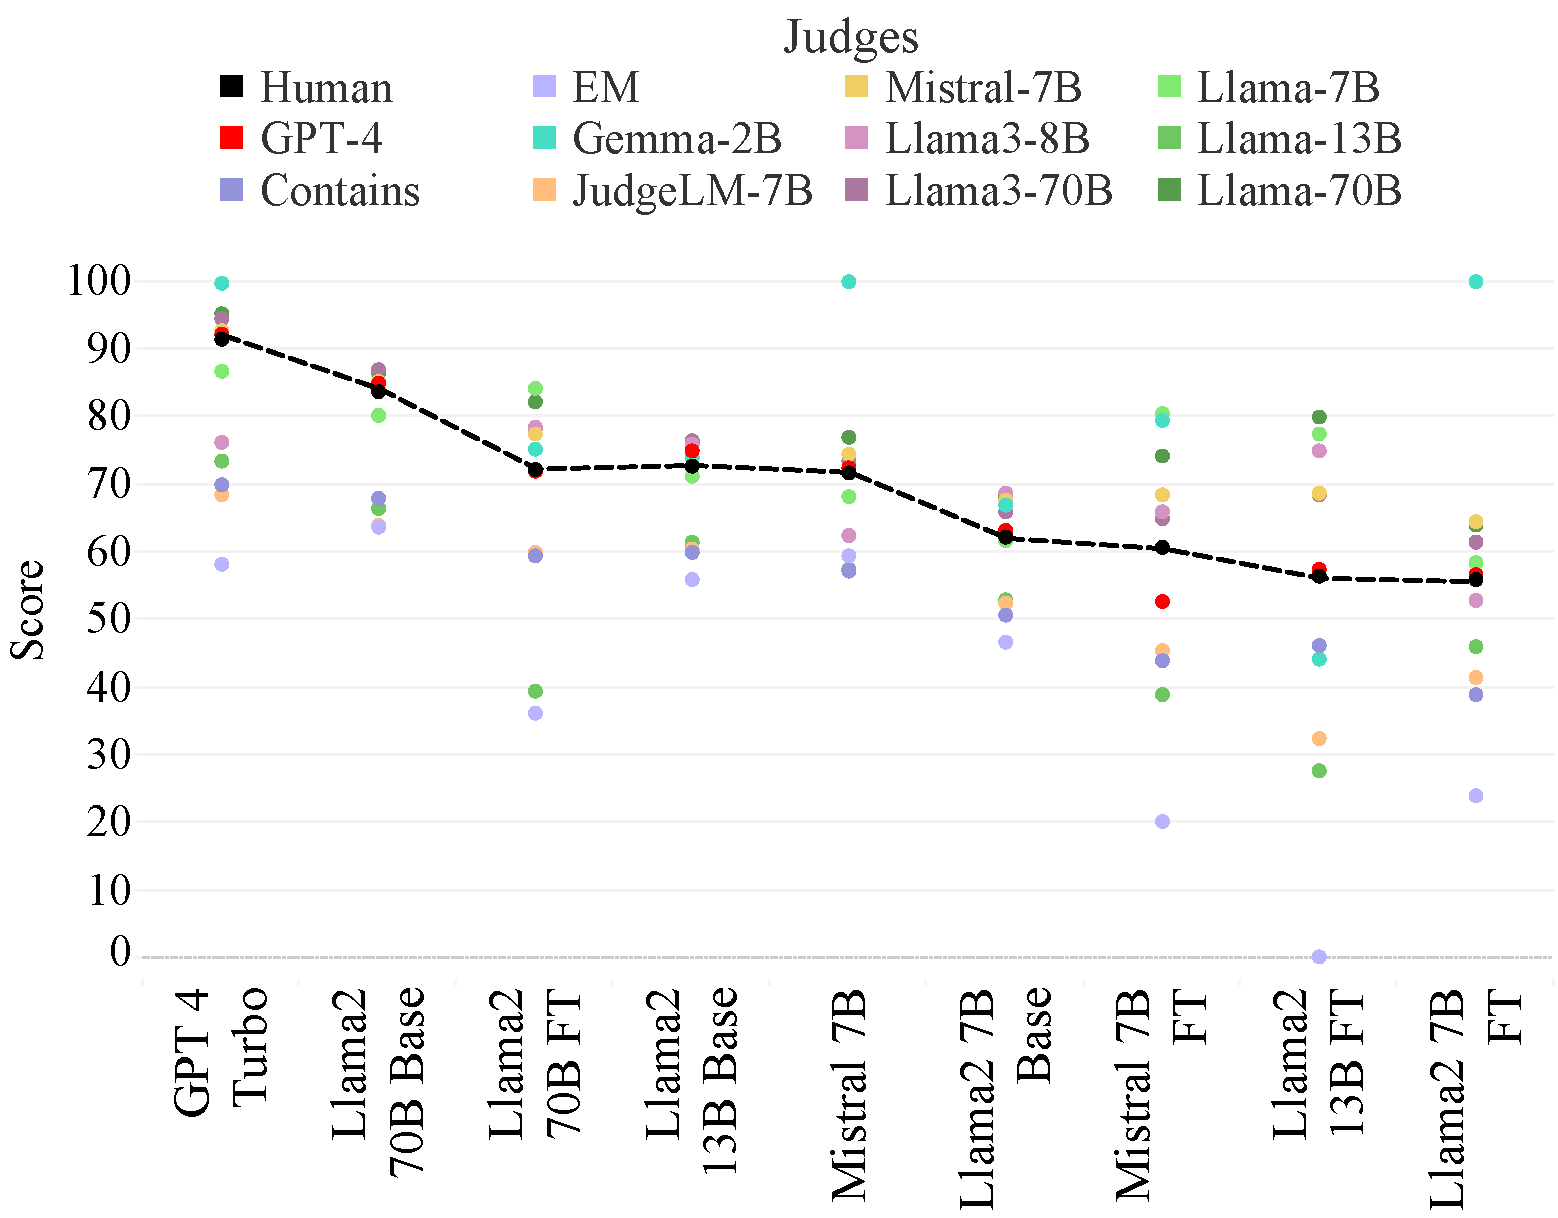
\includegraphics[width=\linewidth]{figures/JudgeScoreforExamTakers.pdf}
        \caption{}
        \label{fig:llmalignment_a}
    \end{subfigure}
    \hfill
    \begin{subfigure}[b]{0.49\textwidth}
        \centering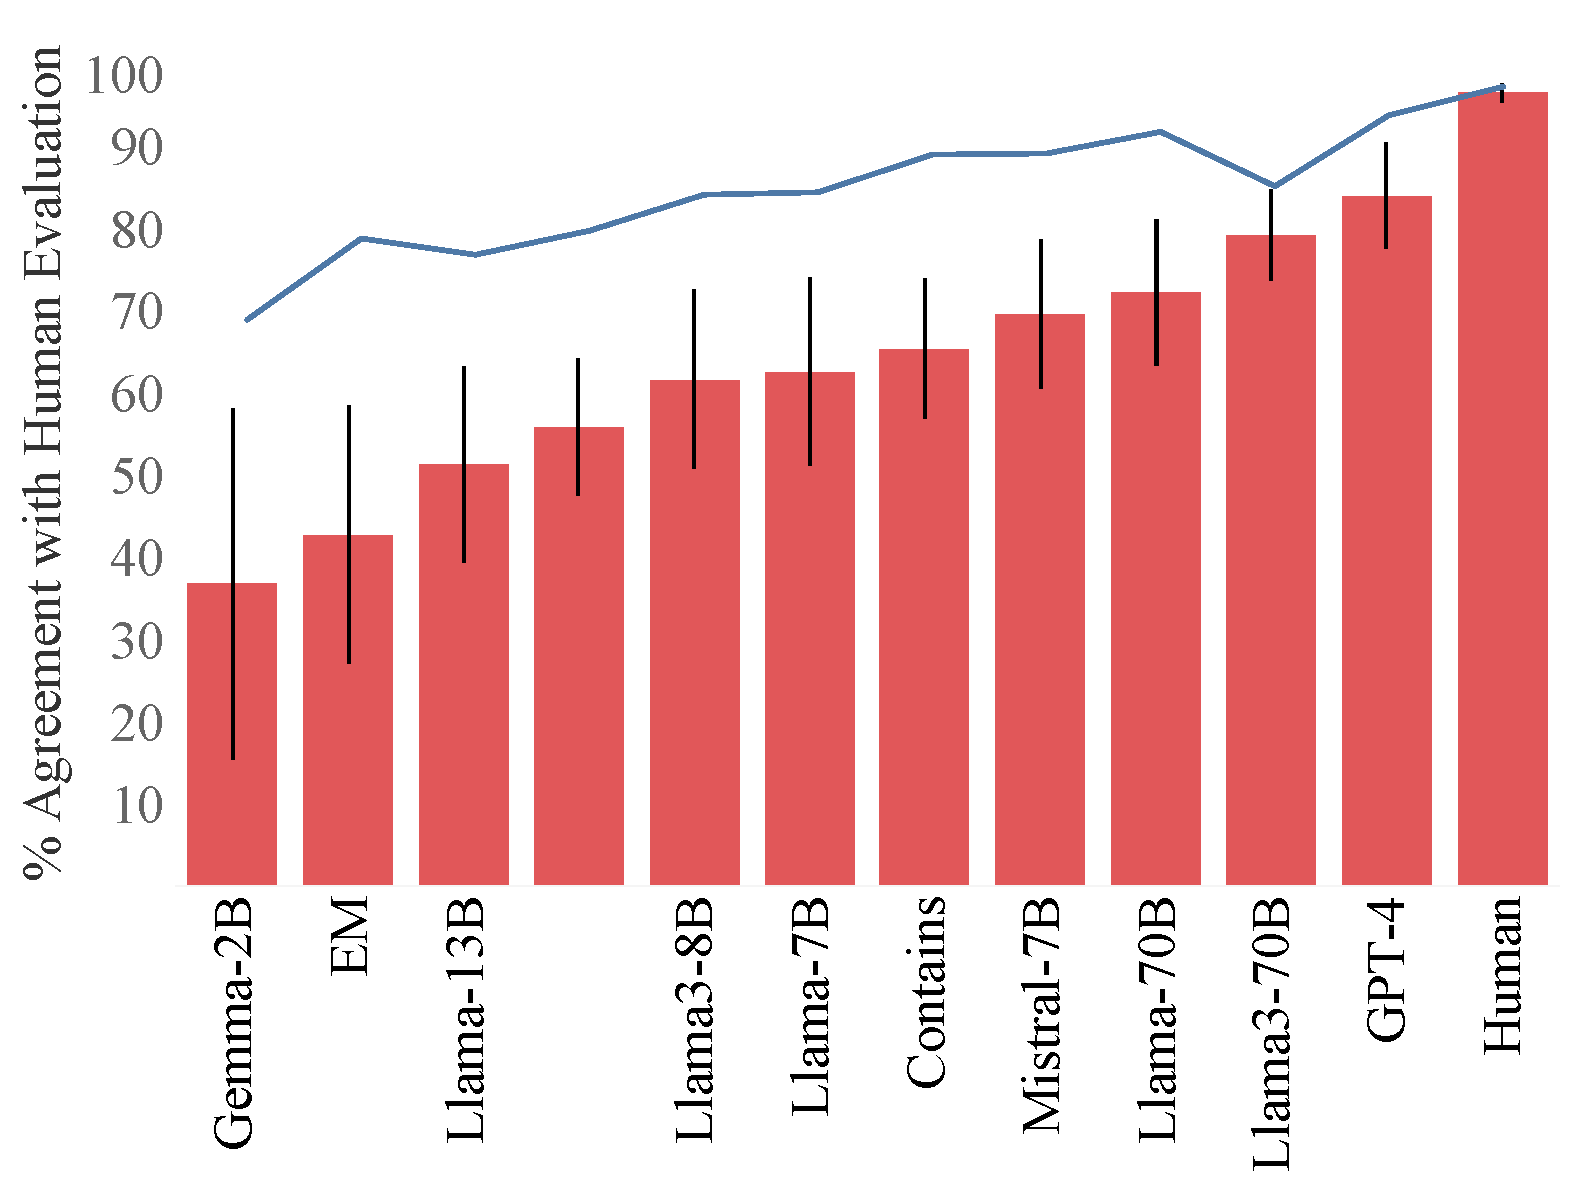
\includegraphics[width=\linewidth]{figures/LLMAlignmentV5.pdf}
        \caption{}
        \label{fig:assigned_scores}
    \end{subfigure}
    \caption{\Judgemodel alignment with human judgment, averaged across \textit{evaluatormodels}. The blue line indicates the percentage of aligned examples, the red bars Cohen's Kappa. 
    Error bars annotate standard deviation across \textit{evaluatormodels}. While alignment is poor for most \Judgemodel, both Llama3 70B and GPT 4 have Cohen's Kappa coefficient that are indicative of excellent alignment (79 and 84\%, respectively). Both of them, however, are still well below the human alignment score, which is 96\%.}
    \label{fig:llmalignment}
\end{figure}





% \subsubsection{Kappa Score vs Evaluation Score}

\paragraph{Kappa vs score}
To get a better idea of how much variation in actual assigned scores can be expected given a particular kappa, we plot the differences between scores provided by judges and those from human assessment across a range of judge kappa scores, in \cref{fig:cohenskappa}.
% \dieuwke{TODO: make y-axis log-scale}.
We can see that for Kappa > 80\%, the evaluation scores of \judgemodels are close to the human evaluation scores for most of the judges, with only up to 5\% difference in their assigned score.
For moderate or slight alignment, we observe a variation of up to 20\% in the evaluation scores for similar kappa alignment.
Furthermore, for several \judgemodels, we observe that the deviation from human-judgements can be quite different for different \evaluatormodels.
In \cref{fig:assigned_scores}, Gemma-2B, for instance, sometimes assigns higher scores than humans, an sometimes much lower.
In the next section, we further explore this particular topic.
\begin{figure}[h]
    \centering
    \begin{subfigure}[b]{0.4\textwidth}
        \centering
        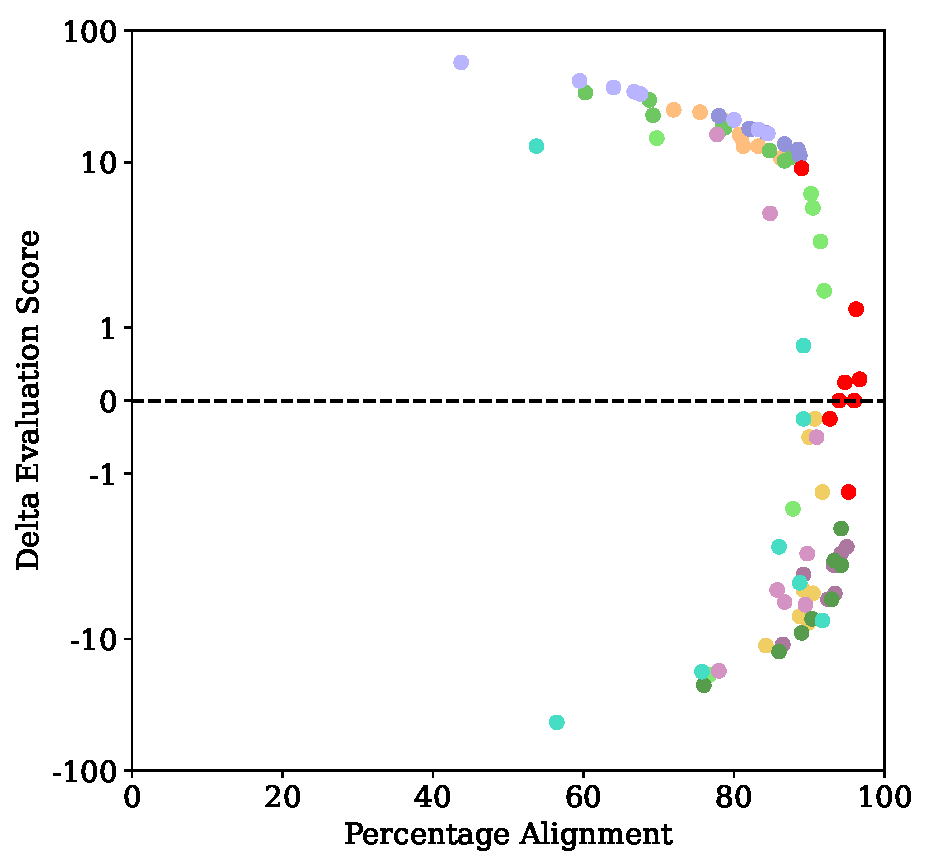
\includegraphics[width=\linewidth]{figures/KappaScoreVariation_V5_a.pdf}
        \caption{}
        \label{fig:cohenskappa_part1}
    \end{subfigure}%
    \begin{subfigure}[b]{0.6\textwidth}
        \centering
        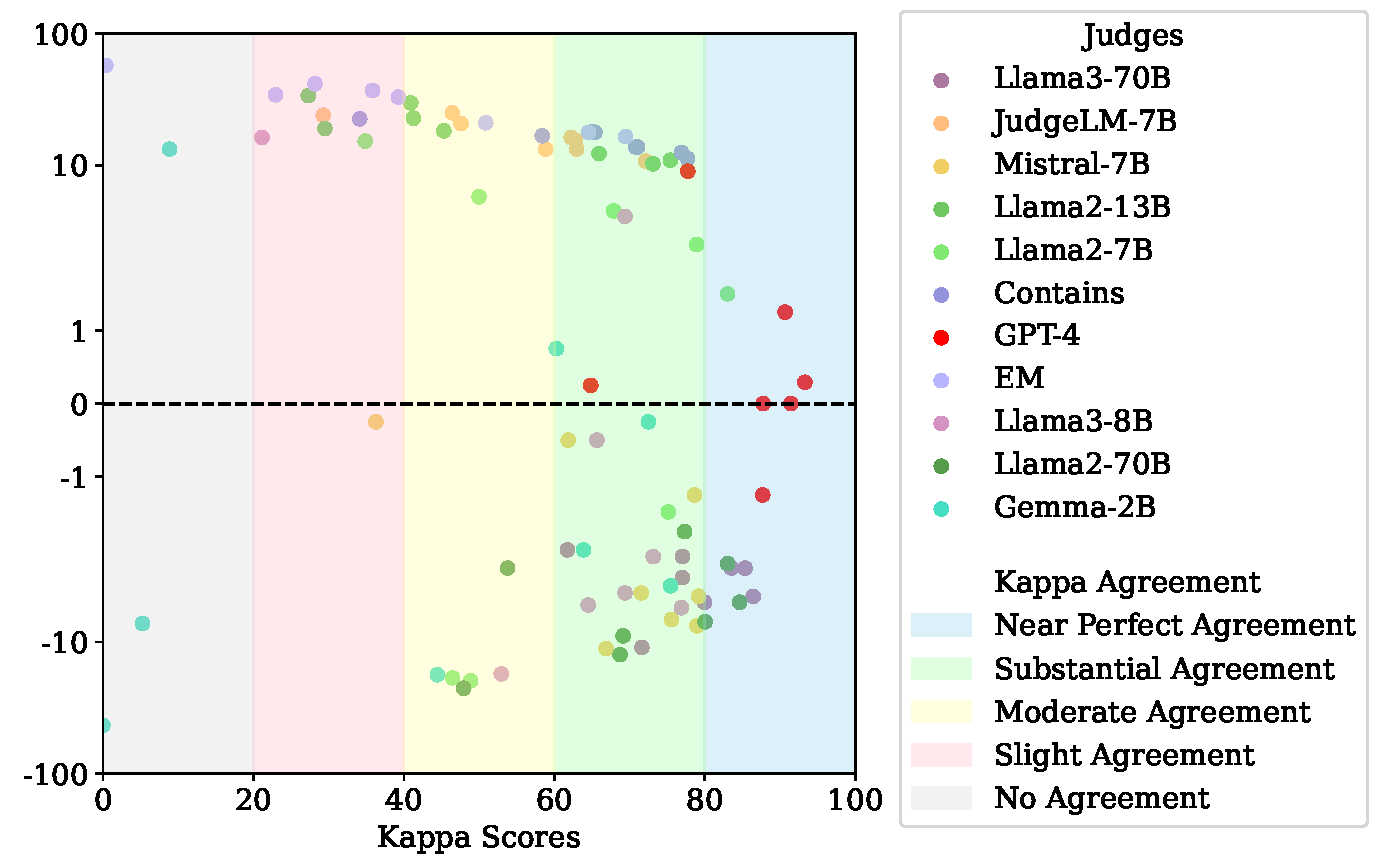
\includegraphics[width=\linewidth]{figures/KappaScoreVariation_V5_b.pdf}
        \caption{}
        \label{fig:cohenskappa_part2}
    \end{subfigure}
    \caption{Delta evaluation score is calculated by taking judge score difference with human judgement. In fig a), we observe skewed distribution for percentage alignment and delta evaluation score while in fig b) we observe that highly aligned LLM judges with kappa > 0.8 exhibit low score variance. Conversely, judges with kappa < 0.8 demonstrate variation, impacting reliability. }
    \label{fig:cohenskappa}
\end{figure}

% \subsection{How does this impact their usability?}
\subsection{Exploring Systematic Patterns in \JudgeModels} \label{sec:results:exploringsystematicpatterns}

% \begin{figure}[h]
%     \centering
%     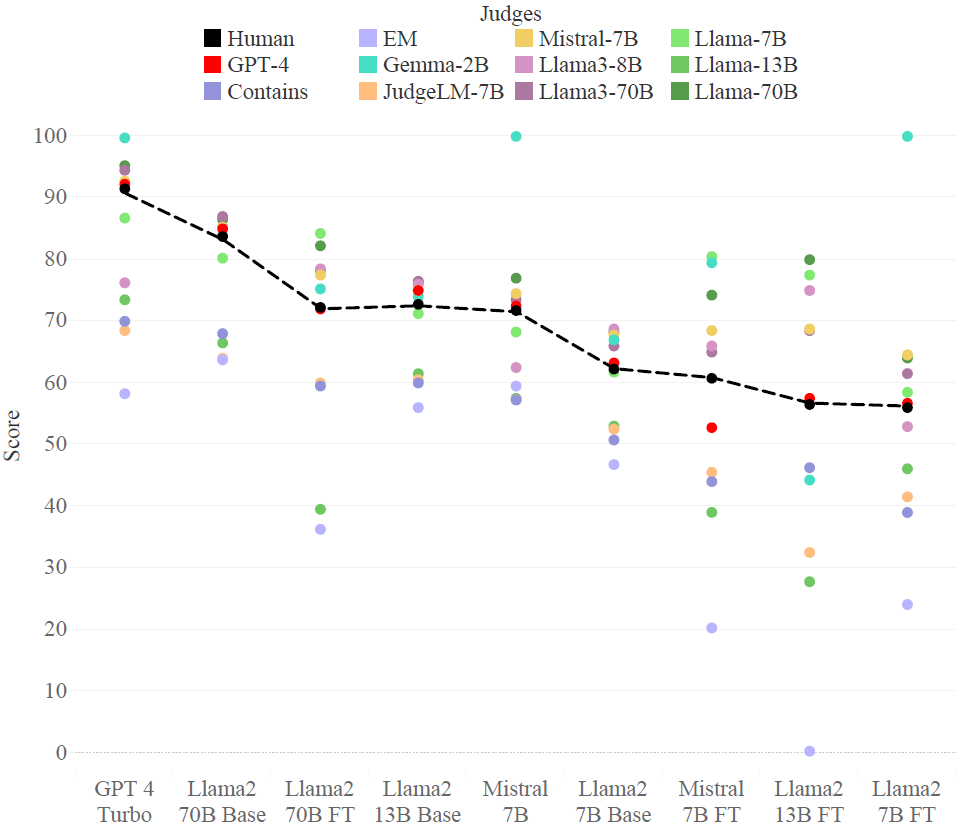
\includegraphics[width=\linewidth]{figures/JudgeScoreforExamTakers.png}
%     \caption{ We plot the delta between Judge exam scores and human assessment for various exam takers.Judge LLMs exhibit diverse distributions and rankings across different exam-taker, none of which exactly mirror the assessments of human judges. However, well aligned tend to consistently score more than the human assessment. \dieuwke{Invert this so that i) the exam taker models are on the y-axis, and the colour indicates the judges, and ii) put the actual score, not the delta.} \dieuwke{Potentially: put next to the figure with the rankings.}}
%     \label{fig:assigned_scores}
% \end{figure}

In the previous section, we have seen that none of the \judgemodels we considered were aligned as well with humans as humans themselves.
Furthermore, as can be seen in \cref{fig:assigned_scores}, the scores assigned by even the best aligned \judgemodels can differ up to 10 points with the human-assigned scores.
However, while this may limit -- to some extent -- the utility of using a \judgemodels to get a perfect estimate of how many of the questions the \evaluatormodels can answer perfectly, the \judgemodels may still offer valuable insights to \emph{differentiate} between different \evaluatormodels.
If judges exhibit systematic biases, such as consistently rating any \evaluatormodel lower -- akin to a very strict teacher -- they will not assign identical scores, but they may assign identical \emph{rankings}.

To evaluate this, we compare the rankings assigned by each \judgemodels to the nine \evaluatormodels (displayed in \cref{fig:rankcorrelation}) and compute their correlation with the human standard. 
In our analysis, it appears that the \eval{Contains} judge demonstrates the highest alignment with a Spearman's rank correlation coefficient ($\rho$) \citep{spearman1904spearman}, maintaining rank consistency across 6 out of 9 examined models. 
Notably, \eval{Contains} performs on par with JudgeLM-7B \citep{zhu2023judgelm}, a language model fine-tuned specifically for evaluating language model responses. 
Following closely behind, GPT-4 and Llama3-70B emerge as the second-best performers. 
Remarkably, while GPT-4 and Llama3 rank the same three models in positions three, four, and five as the human judge, they do so in different orders. 
Despite most judges exhibiting correlations ($\rho$) > 0.7 (\cref{app:correlationcoefftable}), they appear to struggle more in distinguishing between poorer-performing \evaluatormodels compared to better-performing ones.
% We see that all best-aligning judges are consistent in their ranking of the top two models: they all agree that, of the models evaluated, GPT4 is the best performing model, followed by Llama2-70b-base.
% Below the top two, there are more changes.
% The GPT-4 and Llama3 have the same three models in spot three, four and five as the human judge, but both with different orders.
% Generally, judges appear worse at distinguishing poorer performing models than better-performing models.

% Classical lexical models fare even worse with greater misalignment with human judgement across the board, with the -- commonly used -- EM score not even agreeing on the top-performing model.


% \begin{table}[h]
%     \centering
%     \begin{tabular}{|c|c|}
%     \hline
%     \textbf{Model} & \textbf{Spearman Rank Correlation Coeff} \\
%     \hline
%     Human Alignment & 100 \\
%     GPT-4 & 99.17 \\
%     Llama3-70B & 99.17 \\
%     Llama-70B & 81.67 \\
%     Mistral-7B & 77.50 \\
%     Contains & 41.67 \\
%     Llama-7B & 85.00 \\
%     Llama3-8B & 42.50 \\
%     JudgeLM-7B & 59.17 \\
%     Llama-13B & 18.33 \\
%     EM & 65.83 \\
%     Gemma-2B & 48.33 \\
%     \hline
%     \end{tabular}
%     \caption{Judges sorted by Kappa Human Alignment and their Spearman Rank Correlation Coeff}
%     \label{tab:scores_multiplied}
% \end{table}
\begin{figure}[h]
    \centering
    \begin{minipage}[b]{0.44\textwidth}
        \centering
        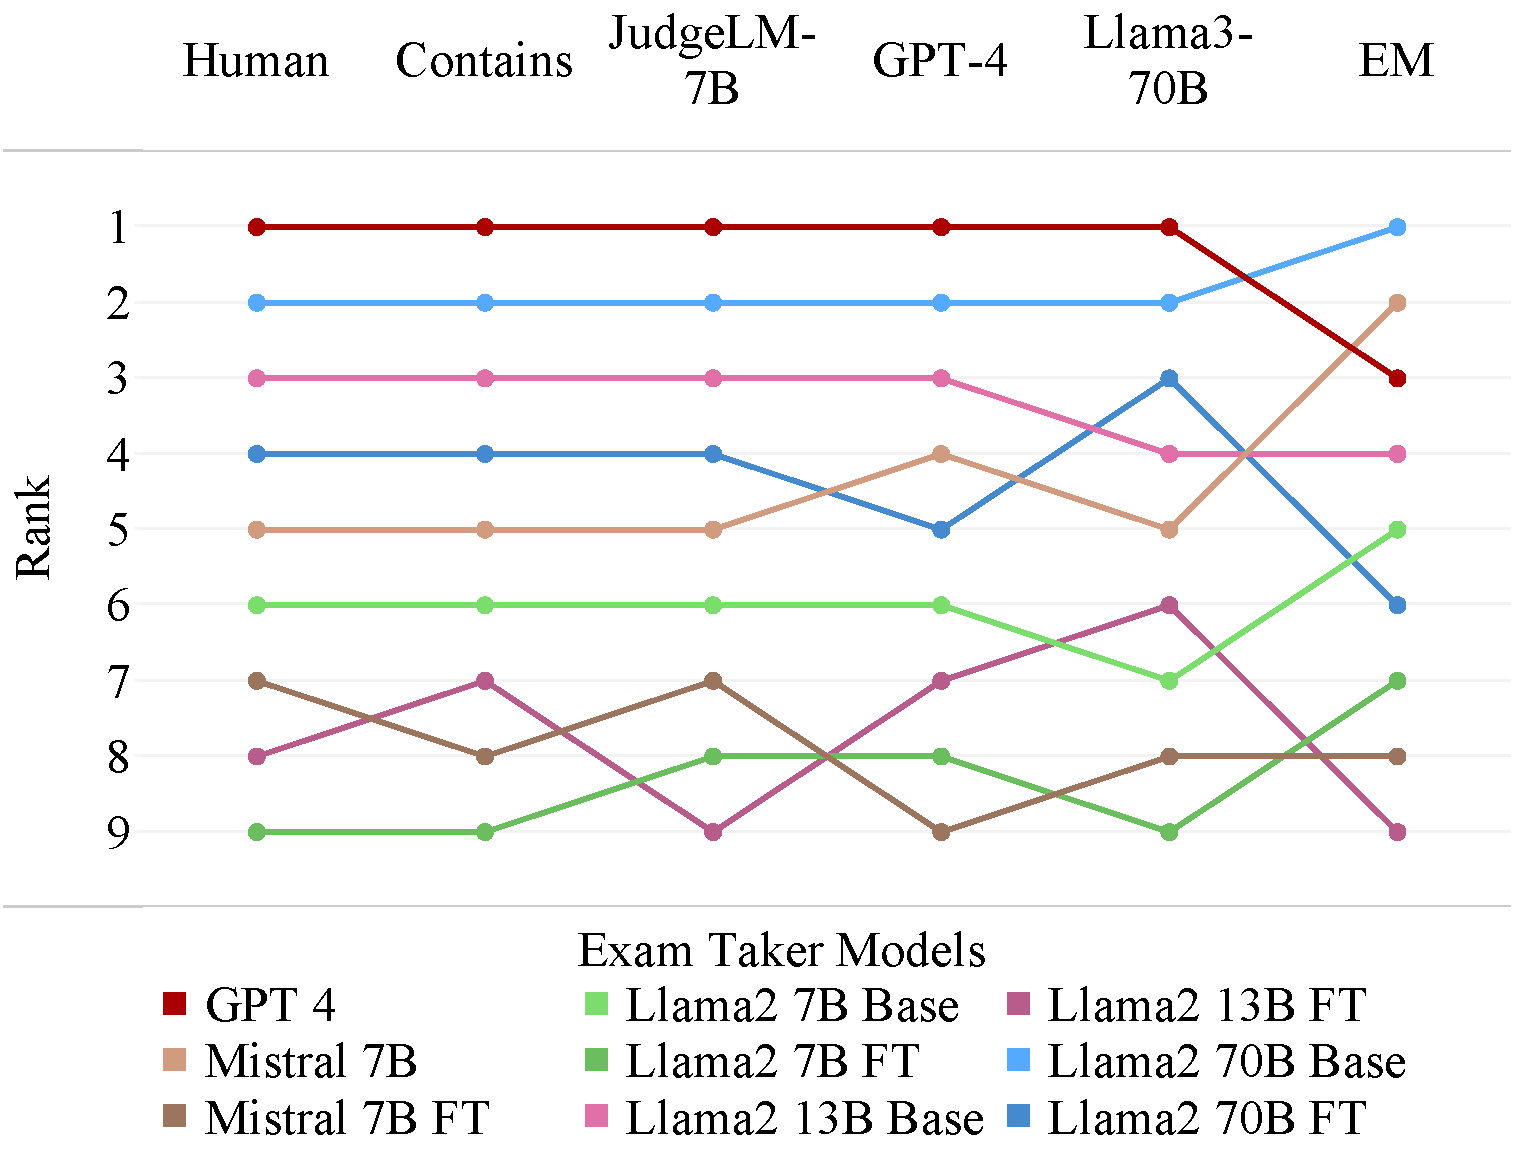
\includegraphics[width=\linewidth]{figures/RankOfEvaluationModels_V3.pdf}
        \caption{\eval{Contains} and \eval{JudgeLM} holds strong with a 67\% Human Assessment ranking retention, closely followed by GPT-4 and LLama3-70B. Notably, distinguishing between poor performing exam taker models presents a challenge for judges across the board}
        \label{fig:rankcorrelation}
    \end{minipage}
    \hfill
    \begin{minipage}[b]{0.54\textwidth}
        \centering
        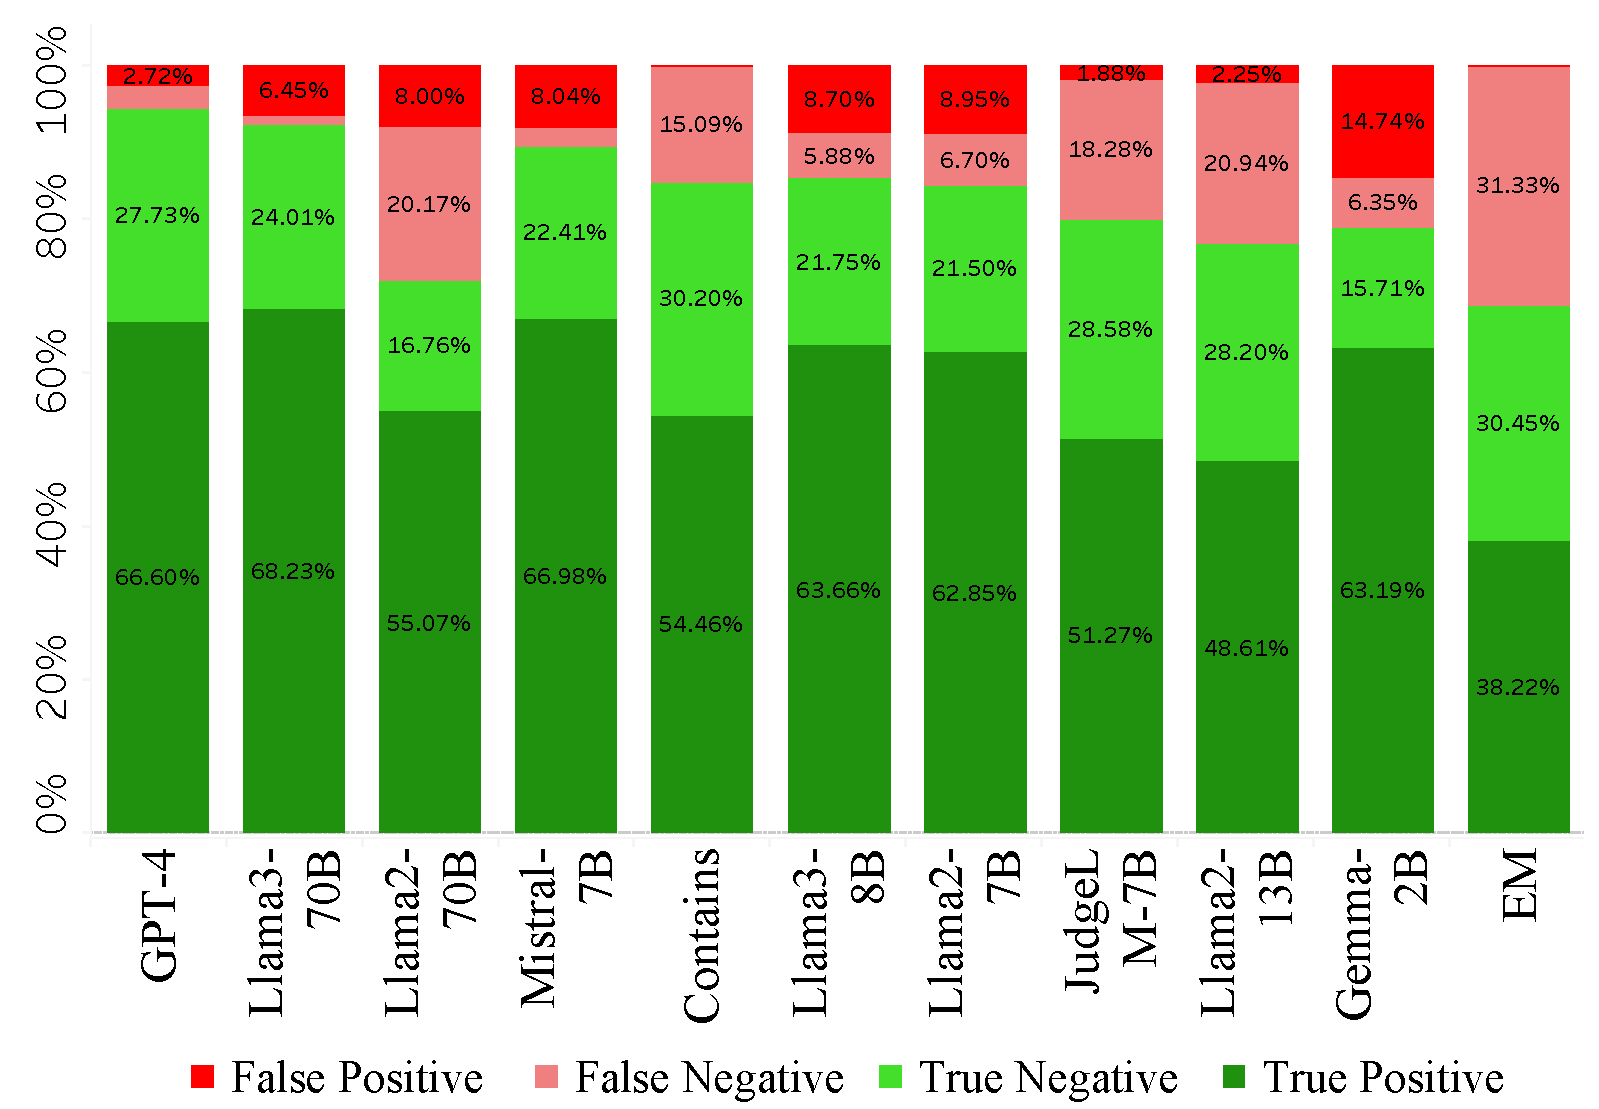
\includegraphics[width=\linewidth,height=5.7cm]{figures/ConfusionMatrixV4.pdf}
        \caption{false positives and negatives across different \judgemodels, ordered from best human aligned (left) to least human aligned (right). Generally, as alignment decreases, both FN and FP increase. Well-aligned models, however, tend to produce more FN than FP.
        \dieuwke{Should increase the font sizes on this one, put the legends on the top and afterwards align appropriately.}}
        \label{fig:confusionmatrix}
    \end{minipage}
\end{figure}


% \begin{figure}[h]
%     \centering
%     \begin{minipage}[b]{0.49\textwidth}
%         \centering
%         \includegraphics[width=\linewidth]{figures/InterLLMAlignment.png}
%         \caption{Inter Judge Alignment}
%         \label{fig:interllmalignment}
%     \end{minipage}
%     \hfill
%     \begin{minipage}[b]{0.49\textwidth}
%         \centering
%         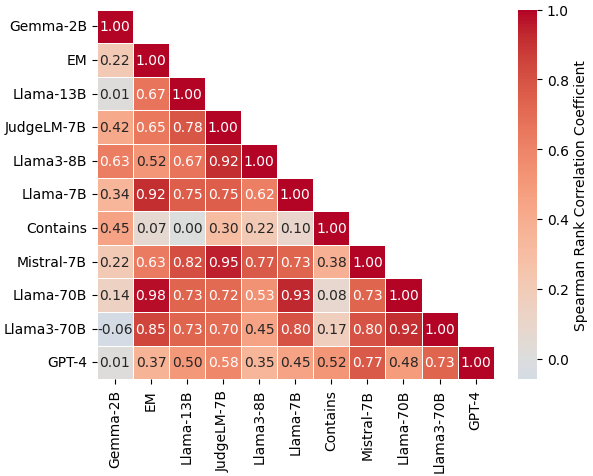
\includegraphics[width=\linewidth]{figures/RankCorrelationCoeff.png} 
%         \caption{Judge Ranking over Evaluation Models}
%         \label{fig:rankcorrelation}
%     \end{minipage}
% \end{figure}

% \subsubsection{Precision, Recall \& False Positives}

% Using the human judgement, we calculate the precision, recall and false positive rate to quantify judge LLM performance. To understand the precision-recall tradeoff, we plot the precision and recall rates and maintain The ordering of LLMs from Figure \ref{fig:llmalignment}. We can observe in figure \ref{fig:precisionrecall}, when LLMs become more aligned with human judgment, their recall improves. Precision, on the other hand, remains relatively consistent across all LLMs due to balancing effect of increase in true positive and false positives. From figure \ref{fig:confusionmatrix}, we can observe increase in true positives but not a similar reverse trend in False Positive. Instead, we see that the False Negatives are decreasing with increase in human alignment for Judges. 

% \begin{figure}[h]
%     \centering
%     \begin{minipage}[b]{\textwidth}
%         \centering
%         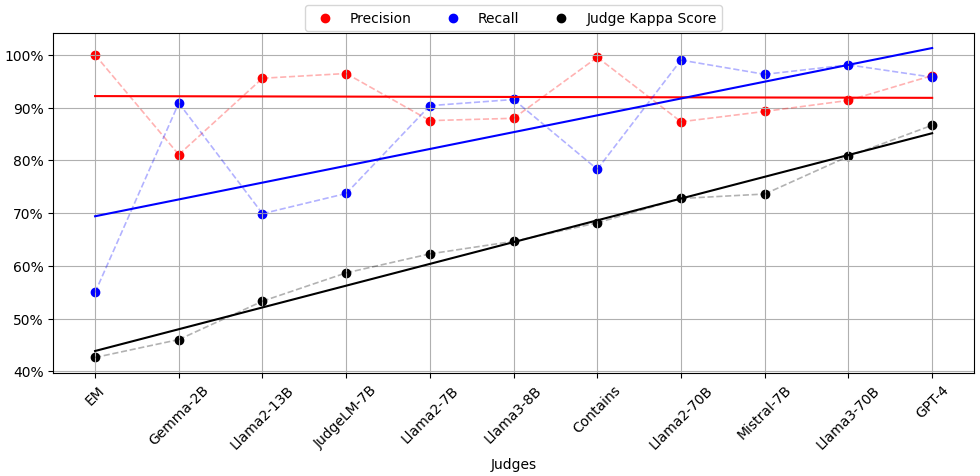
\includegraphics[width=\linewidth]{figures/PrecisionRecall_V4.png}
%         \caption{Precision \& recall with increasing human alignment}
%         \label{fig:precisionrecall}
%     \end{minipage}
% \end{figure}

% \begin{figure}[h]
%     \centering
%     \begin{minipage}[b]{\textwidth}
%         \centering
%         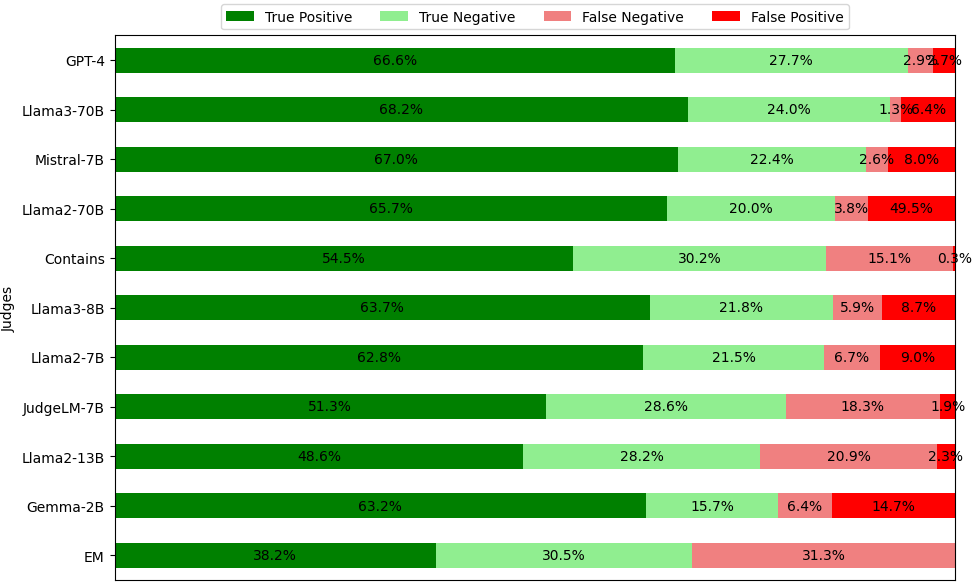
\includegraphics[width=\linewidth]{figures/ConfusionMatrixV2.png}
%         \caption{Judge performance \& error rate with increasing human alignment }
%         \label{fig:confusionmatrix}
%     \end{minipage}
% \end{figure}




% To explore the variability in scores among LLMs within the same cluster, we focus on the first group comprising Llama2-80B, Llama3-80B, Mistral-7B, and GPT-4, plotting their evaluation scores. Figure Y illustrates that despite similar Kappa scores for identical questions and evaluation models, judges' responses yield disparate evaluator results. In the worst-case scenario, these results can differ by up to 10 points

% \begin{figure}[h]
%     \centering
%     \begin{minipage}[b]{\textwidth}
%         \centering
%         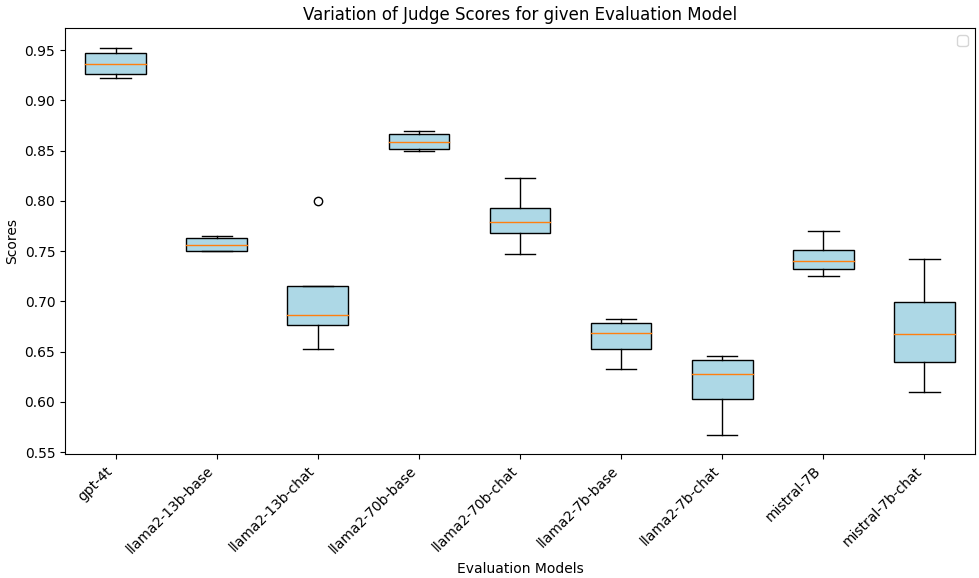
\includegraphics[width=\linewidth]{figures/VariationofScores.png}
%         \caption{Variation of Scores for similar Kappa Scores}
%         \label{fig:llmalignment}
%     \end{minipage}
% \end{figure}

% In our study, we investigated nine evaluation models and anticipated consistency in the ranking of judges across each model. To verify this assumption, we assessed the ranking of each judge across the different evaluation models. Recognizing the possibility of unchanging rankings (no variance), we computed and plotted the Spearman Rank Correlation Coefficient (cite) across the 12 judges. Spearman Rank Correlation is valuable as it gauges the degree to which the relationship between two variables can be described using a monotonic function. A Spearman Rank Correlation exceeding 0.7 indicates a strong correlation, a common occurrence in robust benchmarks. However, the plotted data in Figure (cite) reveals fluctuations in rankings among the remaining evaluators.

% \begin{figure}[h]
%     \centering
%     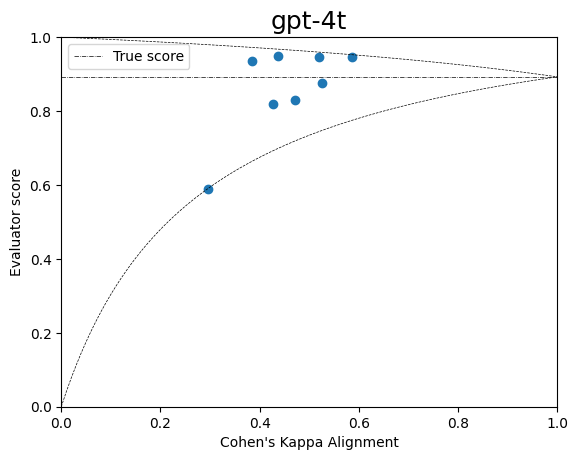
\includegraphics[width=0.6\textwidth]{figures/score-kappa-0.png}
%     \caption{Scores assigned by different evaluators vs their alignment with human evaluations}
%     \label{fig:score-kappa-0}
% \end{figure}

% \begin{figure}[h]
%     \centering
%     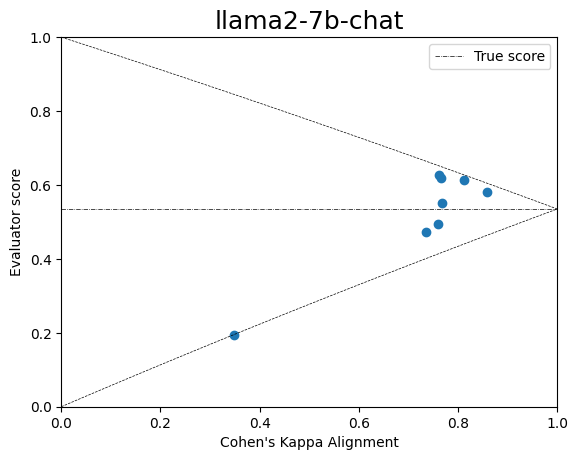
\includegraphics[width=0.6\textwidth]{figures/score-kappa-1.png}
%     \caption{Scores assigned by different evaluators vs their alignment with human evaluations}
%     \label{fig:score-kappa-0}
% \end{figure}

% \begin{figure}[h]
%     \centering
%     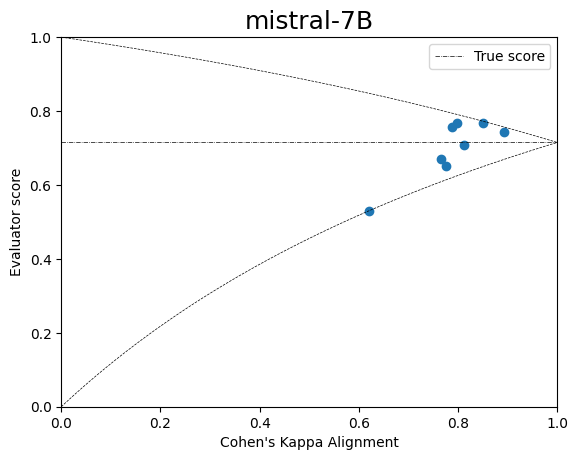
\includegraphics[width=0.6\textwidth]{figures/score-kappa-2.png}
%     \caption{Scores assigned by different evaluators vs their alignment with human evaluations}
%     \label{fig:score-kappa-0}
% \end{figure}





% OLD STUFF


% \begin{figure}[h]
%     \centering
%     \includegraphics[width=\textwidth]{figures/humanalignment_withem.png}
%     \caption{Human Alignment w GT}
%     \label{fig:human}
% \end{figure}

% \begin{table}[h]
%     \centering
%     \caption{Percentage Alignment}
%     \label{tab:my_table}
%     \begin{tabular}{cccccc}
%         \toprule
%         \textbf{Scenario} & \textbf{Avg Alignment} & \textbf{Human-A} & \textbf{Human-S} & \textbf{Human-K} & \textbf{Avg Size} \\
%         \midrule
%         All Questions & 98.33 & 97.33 & 98.5 & 99.17 & 600 \\
%         Low Confidence & 98.92 & 99.51 & 97.7 & 99.53 & 214 \\
%         High Confidence & 98.05 & 96.22 & 98.95 & 98.96 & 386 \\
%         \bottomrule
%     \end{tabular}
% \end{table}

% \begin{table}[htbp]
%     \centering
%     \begin{tabular}{cccccc}
%         \toprule
%         \textbf{Scenario} & \textbf{Avg Alignment} & \textbf{Human-A} & \textbf{Human-S} & \textbf{Human-K} & \textbf{Avg Size} \\
%         \midrule
%         All Questions & 96.75 & 94.81 & 97.08 & 98.38 & 308 \\
%         Low Confidence & 98.92 & 99.51 & 97.71 & 99.53 & 214 \\
%         High Confidence & 92.34 & 85.71 & 95.56 & 95.74 & 94 \\
%         \bottomrule
%     \end{tabular}
%     \caption{Without EM - Percentage Alignment}
%     \label{tab:my_table2}
% \end{table}

% \begin{table}[htbp]
%     \centering
%     \caption{Kappa Scores}
%     \label{tab:my_table2}
%     \begin{tabular}{cccccc}
%         \toprule
%         \textbf{Scenario} & \textbf{Avg Kappa} & \textbf{Human-A} & \textbf{Human-S} & \textbf{Human-K} & \textbf{Avg Size} \\
%         \midrule
%         All Questions & 96.36 & 94.14 & 96.75 & 98.19 & 600 \\
%         All Questions - EM & 92.38 & 88.06 & 92.96 & 96.13 & 600 \\
%         \bottomrule
%     \end{tabular}
% \end{table}

% \begin{figure}[h]
%     \centering
%     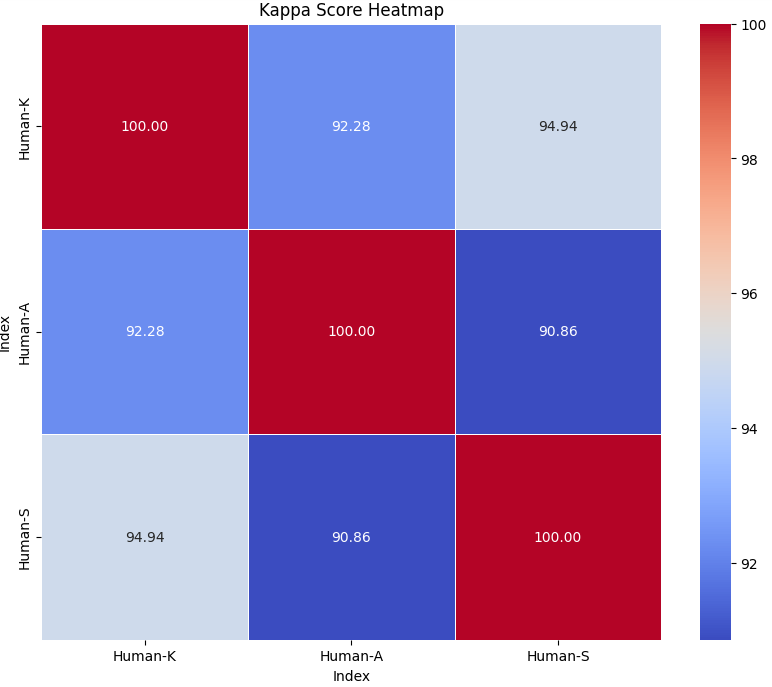
\includegraphics[width=0.8\textwidth]{figures/HumanHeatMap.png}
%     \caption{Human Alignment with Kappa Scores}
%     \label{fig:human}
% \end{figure}

\section {Analysis}\label{sec:analysis}

Next, we conduct multiple case studies aimed at identifying common errors and exposing vulnerabilities in \judgemodels.
Specifically, we study the precision and recall of the \judgemodels (\cref{sec:analysis:subsec:precision_recall}), their ability to recall specific error types (\cref{sec:analysis:subsec:error_analysis}),  the suitability of using \judgemodels for instruction tuned models when compared with base models (\cref{sec:analysis:subsec:basevschat})
% \dieuwke{list what we investigate and provide section numbers}
, how responsive \judgemodels are to the length of prompts and the clarity of guidelines (\cref{sec:analysis:subsec:instructions}) and the leniency of \judgemodels in grading. (\cref{sec:analysis:quantifyingbias}).  
%\dieuwke{insert rest of the results}.

\subsection{Better aligned models have better recall, but not precision}
\label{sec:analysis:subsec:precision_recall}

First, we investigate the precision and recall of the \judgemodels, using the human judgement as gold standard.
We plot both -- maintaining the ordering of \cref{fig:llmalignment} -- in \cref{fig:precisionrecall}.
In the figure, we see that precision stays relatively constant; there is no clear relationship between alignment and how many false positives are predicted, which can be further observed in \cref{fig:confusionmatrix}.
The recall, on the other hand, shows a clear increasing trend: more aligned models have comparatively fewer false negatives.

\begin{figure}[h]
    \begin{subfigure}[b]{0.5\textwidth}
    \centering
        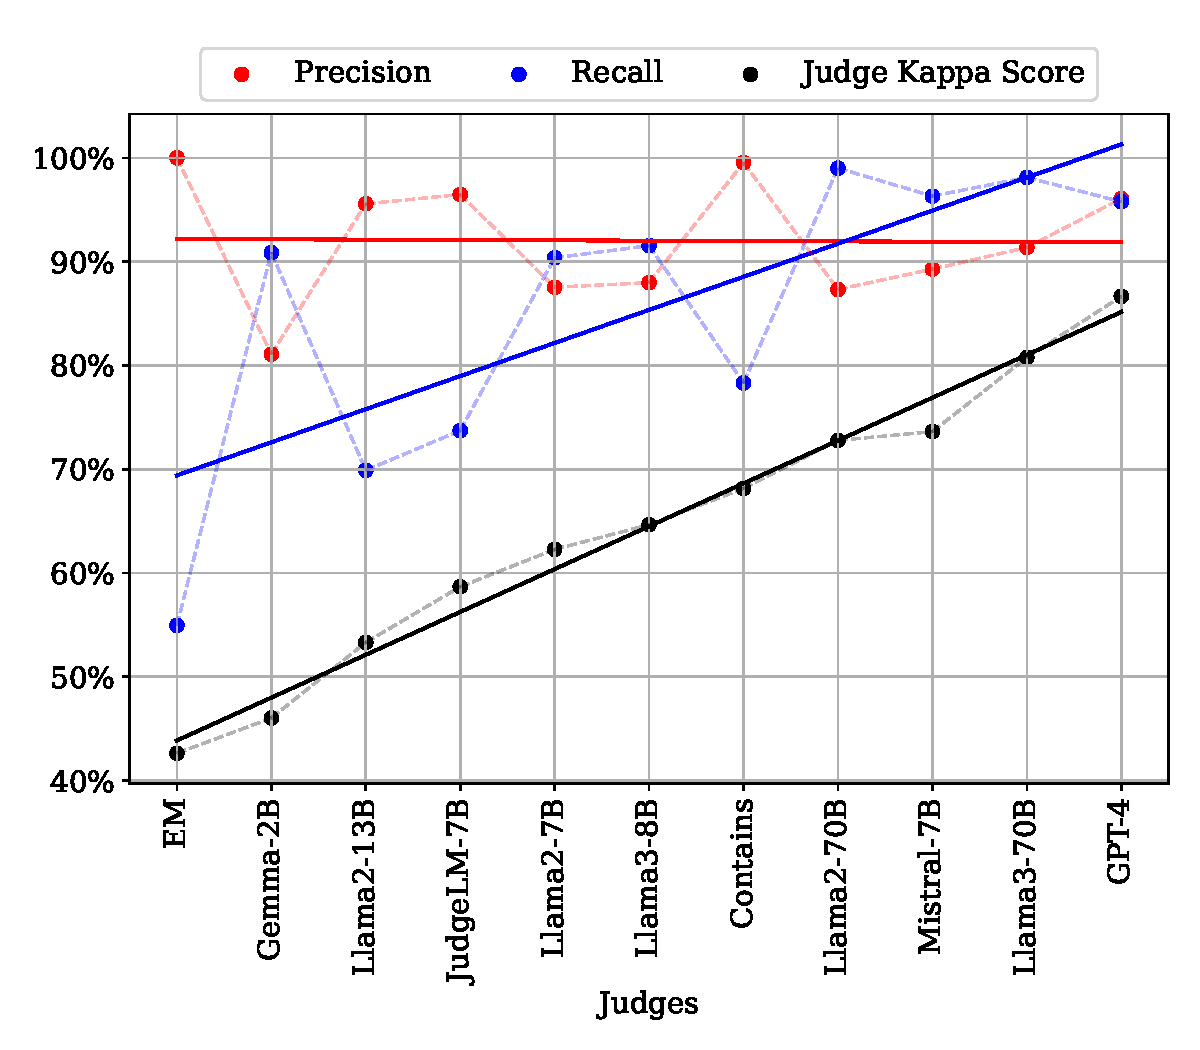
\includegraphics[width=\linewidth]{figures/PrecisionRecall_V5.pdf}
        \caption{}
        \label{fig:precisionrecall}
    \end{subfigure}
    \begin{subfigure}[b]{0.5\textwidth}
    \centering
        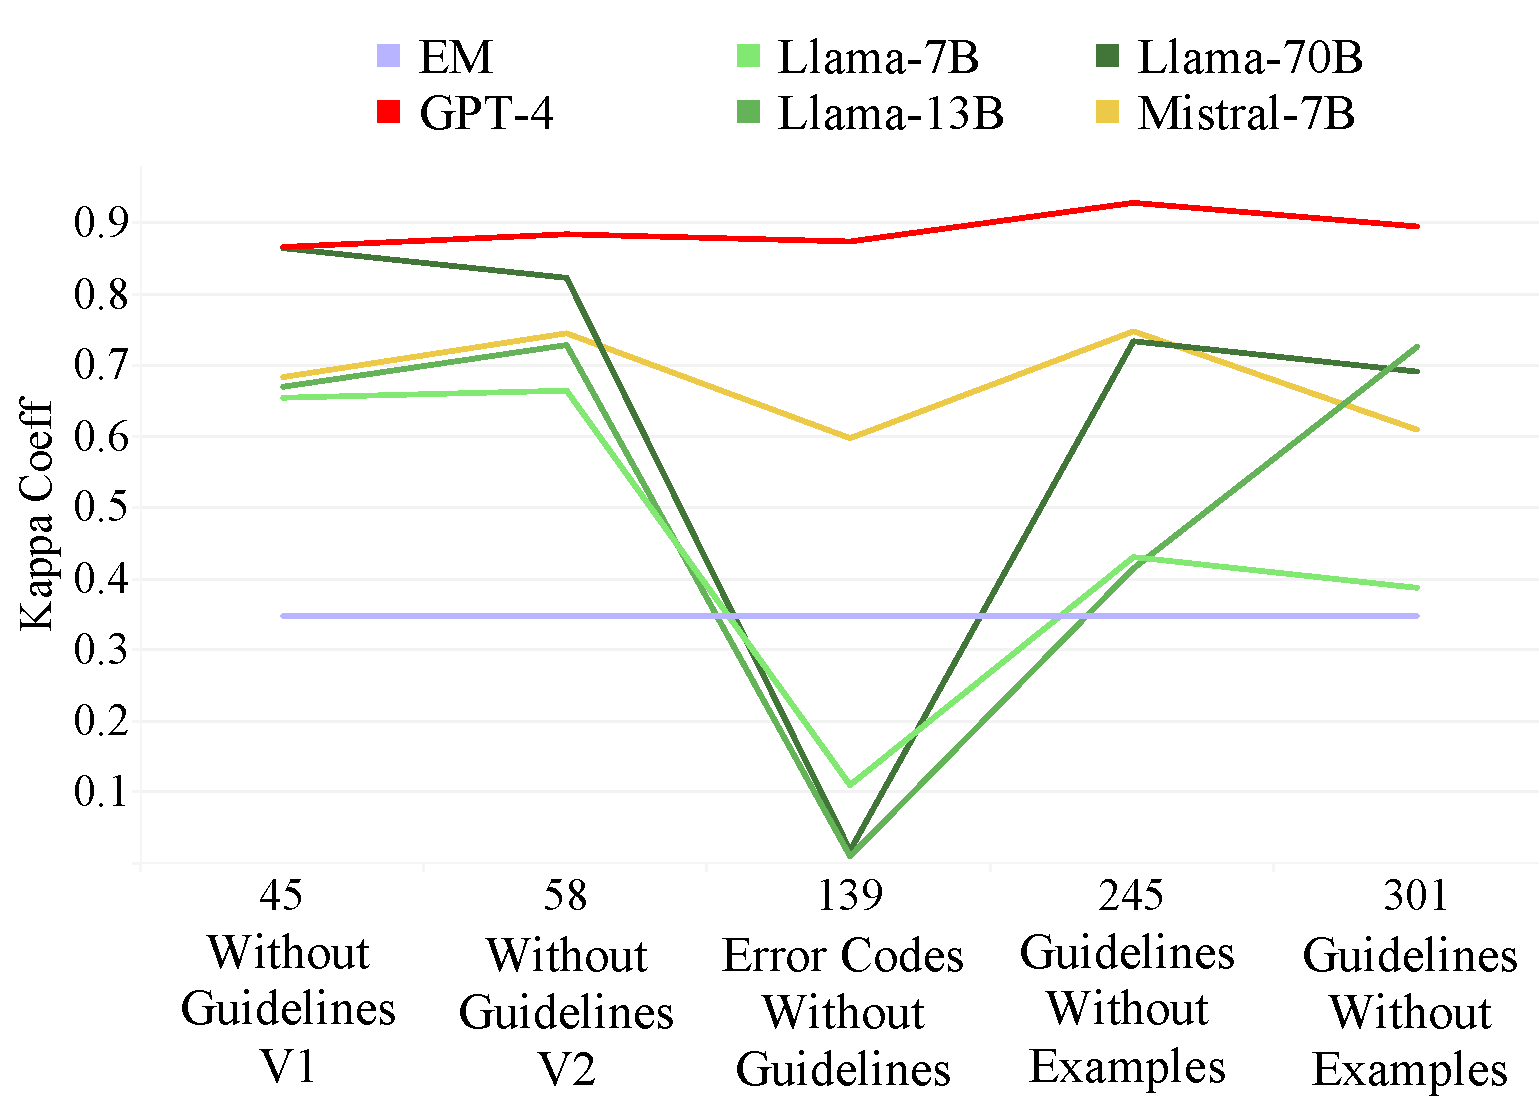
\includegraphics[width=\linewidth]{figures/TooMuchInfo.pdf}
        \caption{}
        \label{fig:TooMuchInfo}
    \end{subfigure}
    \caption{(a) Precision (\( R^2 \) = 0.0003) and recall (\( R^2 \) = 0.55) with increasing human alignment (\( R^2 \) = 0.98) (b) Cohen's Kappa coefficient (human alignment) vs Prompt token size for \JudgeModels
    \dieuwke{Should increase the font sizes on this one, put the legends on the top and afterwards align appropriately.}}
\end{figure}

% \begin{figure}[h]
%     \centering
%         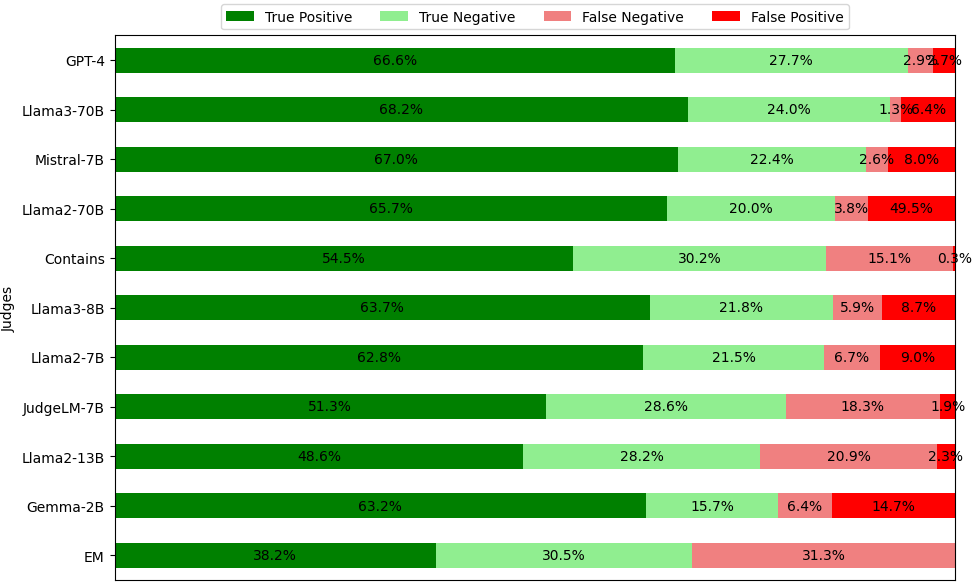
\includegraphics[width=\linewidth]{figures/ConfusionMatrixV2.png}
%         \caption{Judge performance \& error rate with increasing human alignment }
%         \label{fig:confusionmatrix}
% \end{figure}

\subsection{What types of errors do \judgemodels recall?}\label{sec:analysis:subsec:error_analysis}

\begin{table}[ht]
\resizebox{\textwidth}{!}{
    \begin{tabular}{lllll}
        Error code & Explanation & Example & Proportion & GPT-4 Recall\\ 
        \toprule\toprule
        \textbf{Incorrect entity} & \specialcell{Response refers to a wrong entity} & \specialcell{\texttt{Henry VII, Henry VIII, Edward VI,} \\ \texttt{Mary I and Elizabeth I}} & 86.9\% & 84.7\%\\
        \hline
        \textbf{Under-specified} & \specialcell{Response contains only part \\ of the answer} & \specialcell{\texttt{Henry VII, Henry VIII, Edward,} \\ \texttt{Mary, and Elizabeth}} & 10.6\% & 33.9\%\\
        \hline
        \textbf{Too few entities} & \specialcell{Response contains too few entities} & \specialcell{\texttt{Henry VII, Edward VI,} \\ \texttt{Mary I and James I}} & 2.47\% & 67.7\% \\
        \hline
        \textbf{Too many entities} & \specialcell{Response contains too many entities} & \specialcell{\texttt{Henry VII, Henry VIII, Edward VI,} \\ \texttt{Mary I, James I, and Elizabeth I}} & 2.7\% & 84.7\% \\
        \hline
        \textbf{Other} & \specialcell{Response is incorrect but cannot \\ be put into any of the above buckets} & \specialcell{\texttt{I'm sorry but I do not know the} \\ \texttt{answer to that question}} & 1.23\% & 16.9\% \\
        \bottomrule
    \end{tabular}
    }
    \caption{Error codes used to identify the types of errors made by \evaluatormodels when answering questions. The example question in this case is \texttt{``Excluding Lady Jane Grey, who were the five monarchs of the House of Tudor?''}, with the correct answer being \texttt{``Henry VII, Henry VIII, Edward VI, Mary I and Elizabeth I''}}\label{table:error_codes}
\end{table}

Next, we do an analysis of the types of errors that the \judgemodels are making, focusing on the best two \judgemodels: \judge{GPT-4} and \judge{Llama3-70B}.
To do so, we collect 900 outputs of \eval{Llama-7B} and annotate each question with an error code.
Then, we consider what percentage of those types of errors is correctly judged by the two judge models.
An overview of the error codes we considered can be found in \cref{table:error_codes}

In \cref{fig:precisionrecall}, we can see that \judge{GPT-4} has comparatively high recall when the answers refer to an incorrect entity, or too many entities are present.
It's recall for too few entities is also relatively high, while it drops substantially for under-specified answers and other error codes, suggesting that \judge{GPT-4} is more lenient with such mistakes.
\dieuwke{TODO: insert results for Llama3-70-B chat as well.}

% From this case study, we can see that 87\% of incorrect responses were because of knowledge gap of evaluation model. 
% Using GPT-4 Judge LLM, we evaluate each of the responses and then calculate the recall of each error code. From \cref{fig:recallfpr}, we observe that GPT-4 accurately recalls incorrect entities, too many entities, and too few entities. 
% However, GPT-4's recall drops to 20\% - 20\% for underspecified and other error codes indicating that it may be lenient with such error codes.
% 
% \begin{figure}[h]
%     \begin{subfigure}[b]{0.49\linewidth}
%         \centering
%         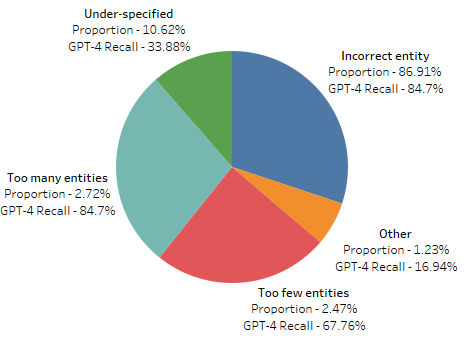
\includegraphics[width=\linewidth]{figures/ErrorCodeAnalysisV2.png}
%         \caption{\judge{GPT-4}}
%         \label{fig:recallfpr}
%     \end{subfigure}
%     \begin{subfigure}[b]{0.49\linewidth}
%         \centering
%         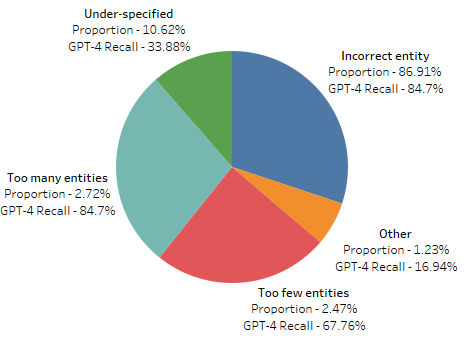
\includegraphics[width=\linewidth]{figures/ErrorCodeAnalysisV2.png}
%         \caption{\judge{Llama3-70B-Chat}}
%         \label{fig:recallfpr}
%     \end{subfigure}
%     \caption{Recall of specific errors by \judge{GPT-4} and \judge{Llama3-70B-chat}. 
%     `Proportion' indicates how many of the observed errors were of that specific type.
%     \dieuwke{Create Llama 3 plot on the right.}}
% \end{figure}

% \begin{figure}
%     \centering
%     \begin{subfigure}[b]{0.42\textwidth}
%         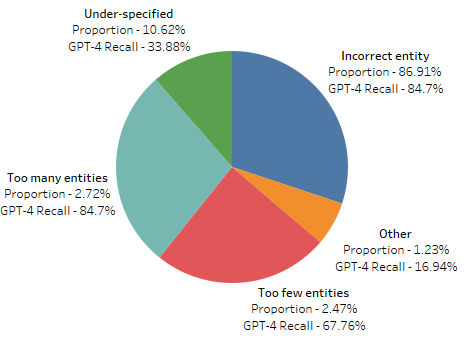
\includegraphics[width=\textwidth]{figures/ErrorCodeAnalysisV2}
%         \caption{}\label{fig:generalisation_over_time_c}
%     \end{subfigure}
%     \caption{}\label{fig:generalisation_over_time}
% \end{figure}

% To understand the pattern in judge LLM incorrect annotations, we run evaluation model Llama-7B on 900 samples and annotate each question with an error code.
% Based on our human annotation guidelines in \cref{sec:experiments:baselineandhumanannotation}, the different error codes are as defined below. 
% We provide examples in \cref{appendix:erroranalysis}. 
% \begin{itemize}
%     \item \textbf{Incorrect entity}: When response is incorrect based on knowledge reasoning.
%     \item \textbf{Under-specified}: When response is incorrect because it has partial information.
%     \item \textbf{Too few entities}: When the response was expected to have multiple entities but LLM responded with only a subset of references.
%     \item \textbf{Too many entities}: When the response was expected to have multiple entities but LLM responded with entities that are not part of the references.
%     \item \textbf{Other}: When response is incorrect but cannot be put into any of the above buckets.
% \end{itemize}

% \begin{figure}[H]
%     \centering
%     \begin{minipage}[t]{\textwidth}
%         \centering
%         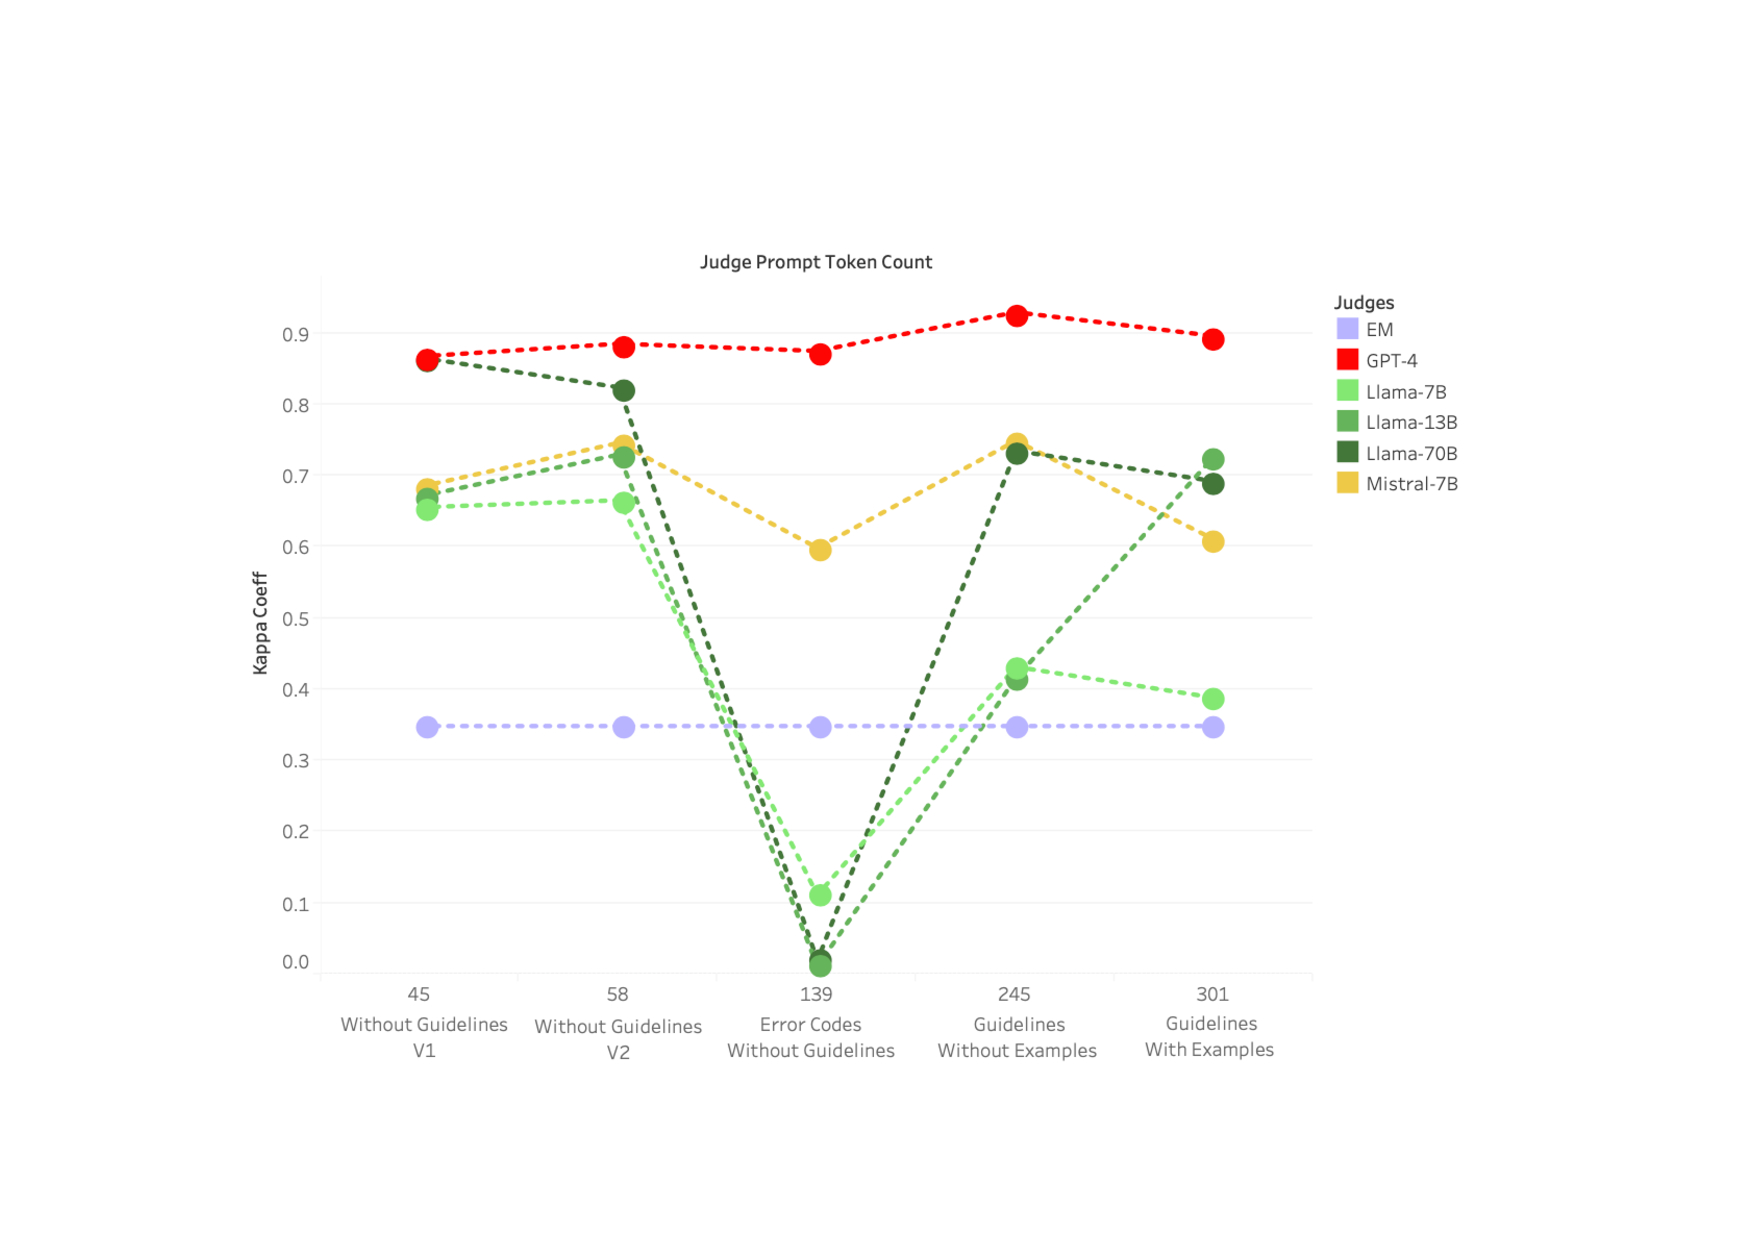
\includegraphics[width=1\textwidth, height=\textheight, keepaspectratio]{figures/TooMuchInfo_Scaled.pdf}
%         \caption{Cohen's Kappa score (human alignment) vs prompt token size for judge LLMs}
%         \label{fig:TooMuchInfo}
%     \end{minipage}
% \end{figure}
\subsection{Base vs Chat analysis} \label{sec:analysis:subsec:basevschat}

% \begin{table}[ht]
% \centering
% \vspace{0.5em} % Adjust the spacing here
% \begin{tabular}{ccccc}
% \multicolumn{1}{c}{\rule{0pt}{1em}} & \multicolumn{1}{c}{\rule{0pt}{1em}\judge{Human}} & \multicolumn{1}{c}{\rule{0pt}{1em}\judge{GPT}} & \multicolumn{1}{c}{\rule{0pt}{1em}\judge{Llama2-70B}} & \multicolumn{1}{c}{\rule{0pt}{1em}\judge{Llama2-7B}}\\ \hline
% \toprule\toprule
% Llama 7B & \rule{0pt}{1em}6.75 & \rule{0pt}{1em}9.5 & \rule{0pt}{1em}4.75 & \rule{0pt}{1em}1.75\\ 
% \midrule
% Mistral 7B & \rule{0pt}{1em}10.75 & \rule{0pt}{1em}11.5 & \rule{0pt}{1em}7.5  & \rule{0pt}{1em}6.25\\
% \midrule
% Llama 13B & \rule{0pt}{1em}16.5 & \rule{0pt}{1em}9 & \rule{0pt}{1em}3.75 & \rule{0pt}{1em}3.75\\
% \midrule
% Llama 70B & \rule{0pt}{1em}10 & \rule{0pt}{1em}10.25 & \rule{0pt}{1em}10  & \rule{0pt}{1em}7 \\
% \bottomrule
% \end{tabular}
% \vspace{1em} % Adjust the spacing between caption and table
% \caption{Difference in Evaluation Scores between different Base - Chat \evaluatormodel pairs for different \judgemodels}
% \label{tab:BasevsChat}
% \end{table}

Here, we examine the differences in evaluation scores between Base and Chat model pairs and how these scores are assessed by different \judgemodels. The results in \cref{tab:BasevsChat} demonstrate that across all \judgemodels, the base models consistently outperform their respective chat \evaluatormodels
 
\begin{table}[ht]
\begin{minipage}[b]{0.49\linewidth}
    \centering
    \renewcommand{\arraystretch}{2.5}
    \resizebox{\textwidth}{!}{ % Adjusts the table to fit the text width
    \begin{tabular}{ | p{2cm} | p{1cm} | p{1cm} | p{1cm} | p{1cm} |}
        \hline
        Judge LLM & Human & GPT-4 & Llama2 & Llama2\\ 
        & & & 70B & 7B\\ \hline
        Llama2-7B & 6.75 & 9.5 & 4.75 & 1.75 \\ \hline
        Mistral-7B & 10.75 & 11.5 & 7.5 & 6.25 \\ \hline
        Llama-13B & 16.5 & 9 & 3.75 & 3.75 \\ \hline
        Llama-70B & 10 & 10.25 & 10 & 7 \\ \hline
    \end{tabular}}
    \caption{Difference in Evaluation Scores between different Base - Chat evaluatormodel pairs for different judgemodels}
    \label{tab:BasevsChat}
\end{minipage}
\begin{minipage}[b]{0.49\linewidth}
\centering
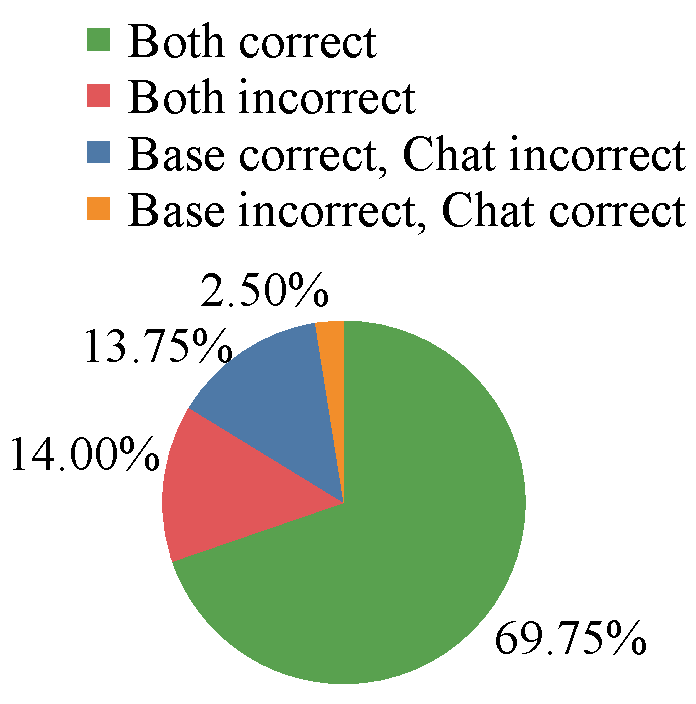
\includegraphics[width=\linewidth]{figures/PieChart.pdf}
\captionof{figure}{Pie chart showing the percentage of questions categorized by the judgement from Base and Chat models.}
\label{fig:comparisonPieChart}
\end{minipage}
\end{table}

% \begin{figure}[H]
%     \begin{subfigure}[t]{0.49\textwidth}
%         % Table LaTeX code
%         \centering
%         \begin{tabular}{ccccc}
%             \multicolumn{1}{c}{\rule{0pt}{1em}} & \multicolumn{1}{c}{\rule{0pt}{1em}\judge{Human}} & \multicolumn{1}{c}{\rule{0pt}{1em}\judge{GPT}} & \multicolumn{1}{c}{\rule{0pt}{1em}\judge{Llama2-70B}} & \multicolumn{1}{c}{\rule{0pt}{1em}\judge{Llama2-7B}}\\ \hline
%             \toprule\toprule
%             Llama 7B & \rule{0pt}{1em}6.75 & \rule{0pt}{1em}9.5 & \rule{0pt}{1em}4.75 & \rule{0pt}{1em}1.75\\ 
%             \midrule
%             Mistral 7B & \rule{0pt}{1em}10.75 & \rule{0pt}{1em}11.5 & \rule{0pt}{1em}7.5  & \rule{0pt}{1em}6.25\\
%             \midrule
%             Llama 13B & \rule{0pt}{1em}16.5 & \rule{0pt}{1em}9 & \rule{0pt}{1em}3.75 & \rule{0pt}{1em}3.75\\
%             \midrule
%             Llama 70B & \rule{0pt}{1em}10 & \rule{0pt}{1em}10.25 & \rule{0pt}{1em}10  & \rule{0pt}{1em}7 \\
%             \bottomrule
%         \end{tabular}
%         \caption{}
%         \label{fig:comparisonTable}
%     \end{subfigure}
%     \begin{subfigure}[t]{0.49\textwidth} % Adjusted width
%         \centering
%         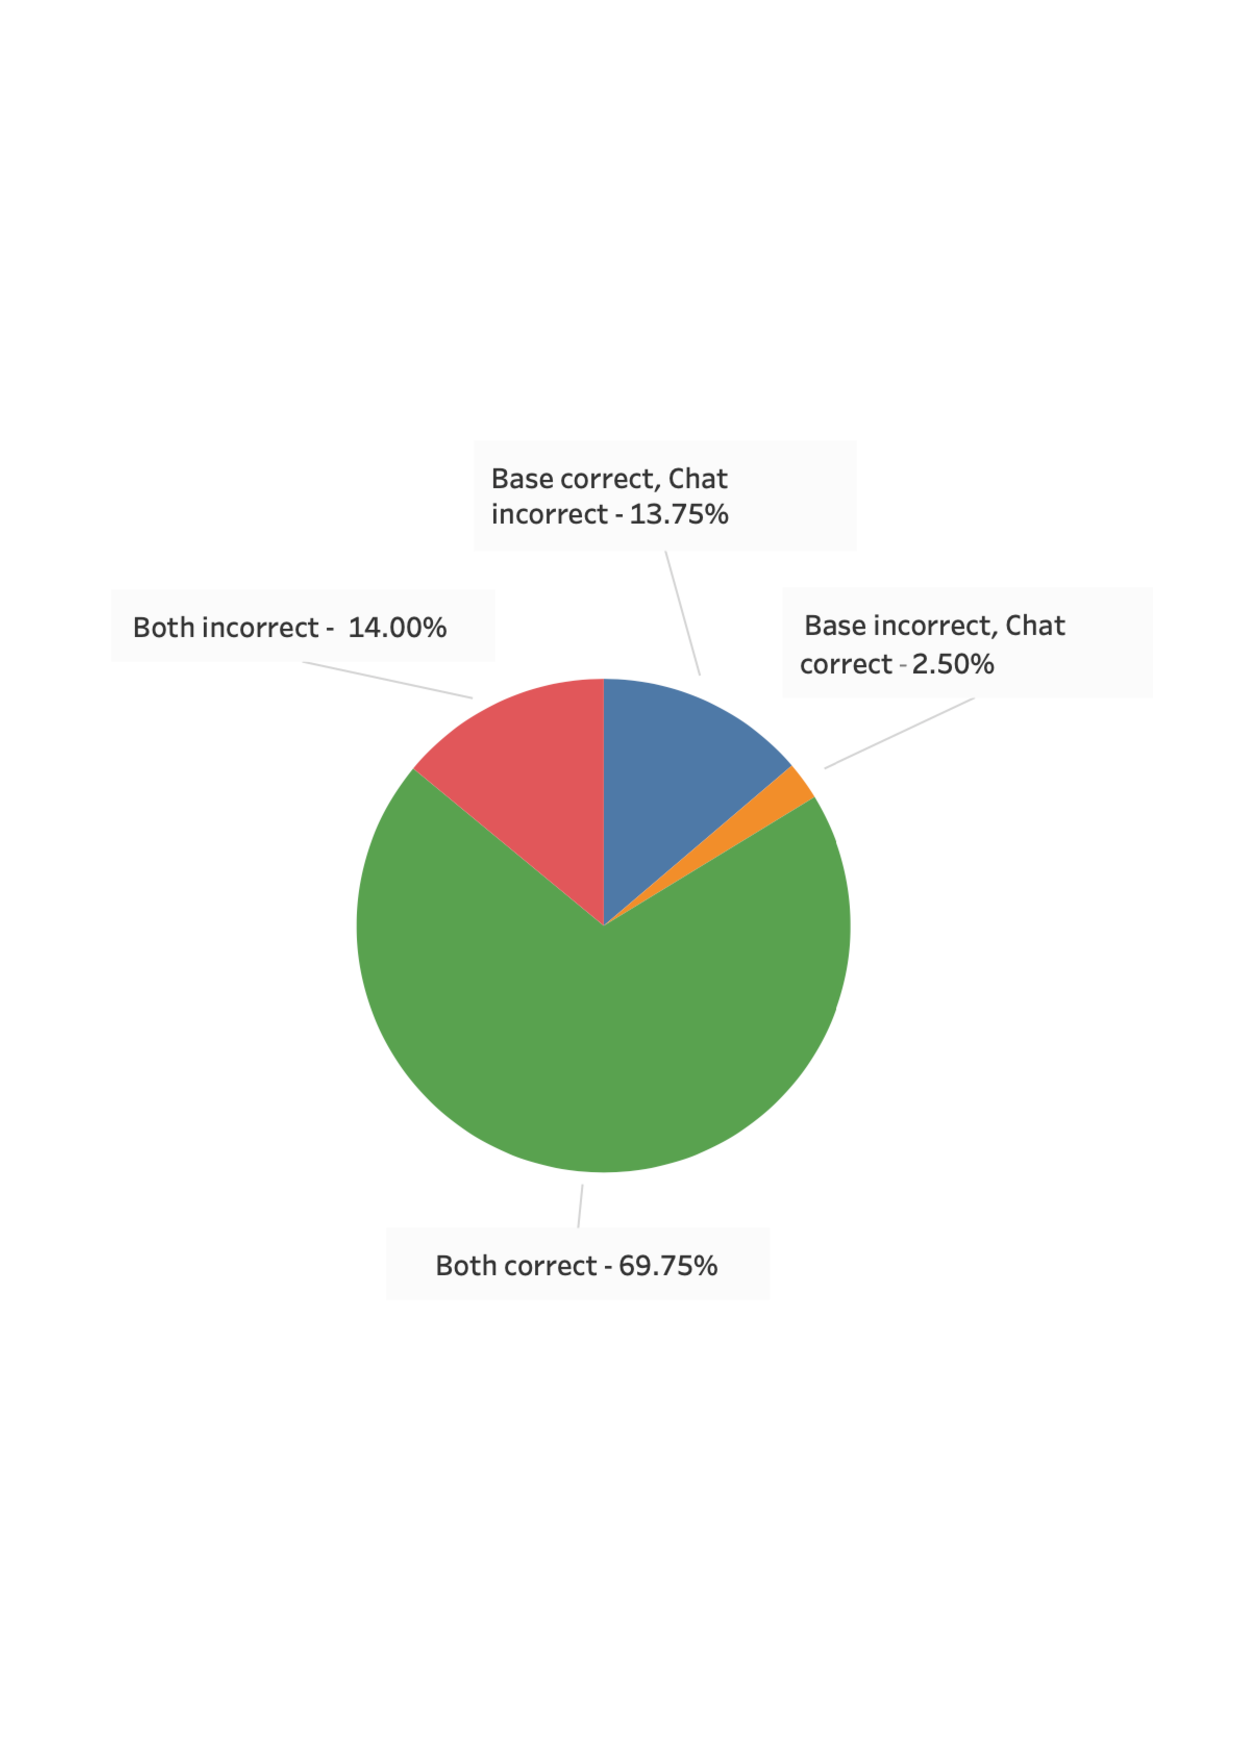
\includegraphics[width=\linewidth]{figures/Error_codes_piechart.pdf}
%         \caption{}
%         \label{fig:comparisonPieChart}
%     \end{subfigure}
%     \caption{(a) Evaluation scores comparison in tabular format for different Base-Chat \evaluatormodel pairs for different \judgemodels. (b) Pie chart showing the percentage of questions categorized by the judgement from Base and Chat models.}
%     \label{fig:BasevsChatErrorPlots}
% \end{figure}
 
% \begin{figure}[H]
%     \begin{subfigure}[t]{0.57\textwidth}
%         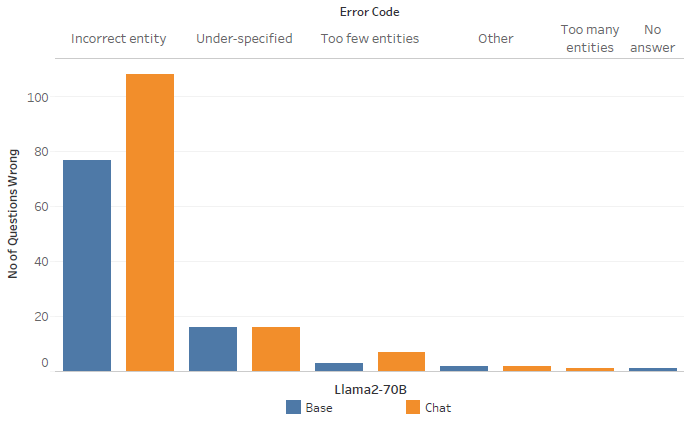
\includegraphics[width=\linewidth]{figures/Error_Codes_BarPlot.png}
%         \caption{}
%         \label{fig:comparisonBarplot}
%     \end{subfigure}
%     \hspace{0.03\textwidth}
%     \begin{subfigure}[t]{0.42\textwidth}
%         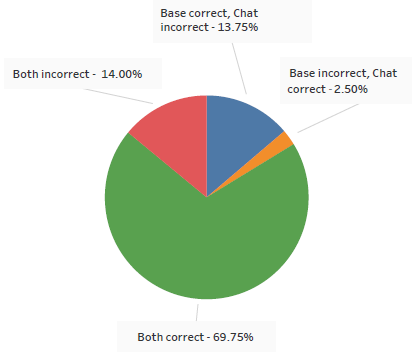
\includegraphics[width=\linewidth]{figures/Error_codes_piechart.png}
%         \caption{}
%         \label{fig:comparisonPieChart}
%     \end{subfigure}
%     \caption{(a)Incorrect questions count by error codes for \eval{Llama2 70B} Base vs Chat models
%     (b) Pie chart showing the percentage of questions categorized by the judgement from Base and Chat models.}
%     \label{fig:BasevsChatErrorPlots}
% \end{figure}

Let us assume the difference in the score of Base and Chat models is because of the following factors:

\begin{itemize}[noitemsep]
\item Knowledge unlearning by the chat models or Loss in knowledge (Correct Answer by Base model and Wrong Answer by Chat model) - $\mathcal{L}_{knowledge}$
\item Error in judgement by \judgemodels (Right answer by Chat model but wrong judgement or Wrong answer by Base model but judged as right) - $\epsilon$
\item Misc (Chat model fails to understand the prompt or answer Cut off) - $\mu$
\end{itemize}

\[
\begin{array}{cc}
\Delta_{\text{Human}} = \mathcal{L}_{knowledge} + \mu & \hspace{2cm} \Delta_{\text{LLM}} = \mathcal{L}_{knowledge} + \mu \pm \epsilon
\end{array}
\]

%%%%%%%%%%%%%%%%%%%%%%%%%
% Storyline
% 1) First we show the difference in scores and show not many 'Answer cut off' or other errors for chat models and hence its mostly Knowledge unlearning that contributes to delta in scores between Base and Chat models
% 2) Then we have to explain why is the delta varying across all judge models since Knowledge unlearning is same no matter what judge model we use. So here we say that its upto the judge model. Bigger judge = lineant scoring, smaller judge = harsher. Hence decrease in delta. Additionally, Knowledge unlearning is greater in bigger Base-Chat pairs
%%%%%%%%%%%%%%%%%%%%%%%%%%

Assuming there is zero error in human judgement, $\epsilon$ in $\Delta_{\text{Human}}$ = 0. 

The plots in \cref{fig:comparisonPieChart} and \cref{fig:comparisonBarplot} suggest that there is some knowledge unlearning, as the Chat model provides more incorrect answers than the Base model, with the majority of these errors being classified as 'incorrect entities' or 'under specification'. Examples can be found in \cref{app:BaseVsChatSupp}

Furthermore, \cref{fig:BasevsChat} shows with an increase in model size, \judge{GPT} has a similar Kappa and alignment score with humans only for the Chat models. This implies that while bigger \judgemodels effectively parse and evaluate the verbose responses from the chat models, the main problem lies in the accuracy of their answers, which leads to a lower judge score and further suggesting knowledge unlearning.

% and the knowledge gap between the base and chat models is increasing with increase in \evaluatormodel size
% The absolute $\Delta_{\text{LLM}}$ and $\Delta_{\text{Human}}$ values increase as the \evaluatormodels size increases. However the knowledge gap between the Base-Chat pairs of larger models is greater than for smaller models.
Interestingly, across all \judgemodels, as the size of the \evaluatormodel increases, $\Delta$ also increases, suggesting that $\mathcal{L}_{knowledge}$ between the Base and Chat models widens as the model size grows.
% This discrepancy underscores the inadequacy of smaller \judgemodels as evaluators

Additionally, as the \judgemodel size gets smaller, the $\Delta_{\text{LLM}}$ values decreases, well beyond the observed $\Delta_{\text{Human}}$. Given that $\mathcal{L}_{knowledge}$ and $\mu$ remain constant across all the \judgemodels, the only variable changing here is $\pm \epsilon$. \cref{tab:eval-scores} reveals that both base and chat models are evaluated too strictly by the smaller \judgemodels, resulting in $\Delta_{\text{LLM}}$s that are smaller but absolute scores that deviate significantly from the true scores. 


\begin{figure}[h]
    \centering
    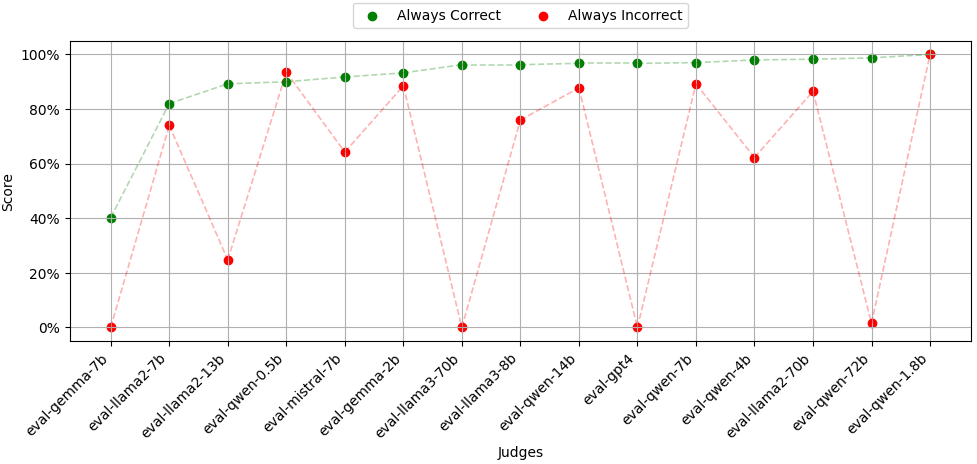
\includegraphics[width=\textwidth]{figures/Judgeguidelines.png}
    \caption{Performance of \judgemodels with constant response outputs \kc{Fig to be updated}}
    \label{fig:judge_dummy}
\end{figure}

% \begin{figure}[H]
%     \begin{minipage}[b]{0.49\textwidth}
%         \centering
%         \includegraphics[width=\textwidth]{figures/BasevsChat7b.png}
%         % \caption{Comparison Scores for Llama 7B Base and Llama 7B Chat}
%     \end{minipage}
%     \hfill
%     \begin{minipage}[b]{0.49\textwidth}
%         \centering
%         \includegraphics[width=\textwidth]{figures/BasevsChat70b.png}
%         % \caption{Comparison Scores for Llama 70B Base and Llama 70B Chat}
%     \end{minipage}
%     \caption{Comparison of Llama 7B and Llama 70B Models}
%     \label{fig:comparison}
% \end{figure}



% From these observations, we can draw the conclusions that

% 1) There is a knowledge gap between base and chat models which gets more prominent in bigger models. \\
% 2) The ideal LLM evaluator is more lenient than the smaller models and more stricter than GPT \\
% 3) Base models are subject to more relaxed judgement as compared to Chat models.

\subsection{\JudgeModel sensitivity to prompt length and quality}\label{sec:analysis:subsec:instructions}

% \textcolor{red}{Update with latest experiment V3-V4-Default-V2-V 1 trends. Bake everything into 1 plot.}
% \dieuwke{I am a bit confused about this subsection, to be discussed!}

Next, we study the impact of the prompt to the \judgemodels' ability to do accurate assessment.
Specifically, we investigate to what extent the precise instructions provided to the \judgemodel impact how it judges \evaluatormodels' answers.

We use five different prompt versions varying in length and specificity, with token counts excluding those from the question and references, focusing only on the instructions given to the \judgemodel during evaluation (see \cref{app:TMI} for prompt templates). Each prompt instructs the \judgemodels on evaluating responses, with complexity and detail increasing with token count. Error codes are introduced in the third smallest prompt (139 tokens, see \cref{app:error_codes_without_guidelines}) and elaborated with examples in the longer prompts.
% 
% \dieuwke{We need a bit more explanation of where these prompts come from and how they differ, plus a link to the full prompts in the appendix.}
% The aim was to observe how these variations affected the stringency of evaluation and to evaluate the sensitivity of the Judge LLM's performance to the prompt. 
% \textcolor{red}{Let's remove Llama 13B now as it's making the graph confusing}\\
% \textcolor{red}{Key Takeaway - Adding more instructions for Judges makes them more lineant}
% With an increase in the number of tokens in the prompt, resulting in higher complexity and detailed instructions for the judge to follow, the agreement between the judge LLM and human evaluation tends to decrease, as measured by the Cohen's Kappa score. 
% However, this trend does not apply to GPT-4, which maintains a high level of agreement with human evaluation even as the prompt complexity increases, and in fact gets a higher alignment with better instructions.

% For Human Guidelines V3, there is a decline in alignment as the prompt introduced the different types of errors that the judge could encounter,but without proper explanation that confused all the judge LLMs. However, in the subsequent bigger prompts, each error type was elaborated with examples to clear any ambiguity for the judge LLMs, which lead to a better performance.

From \cref{fig:TooMuchInfo}, it is evident that both \judge{Mistral-7B} and \judge{GPT-4} exhibit little variance in their Kappa agreement with humans based on the level of detail in the evaluation guidelines provided in the prompt. However, all the \judge{Llama-2} models perform worse as the prompt length and guideline complexity increase.

The \judgemodels are sensitive to the prompt. Prompt engineering to improve the evaluation performance of the \judgemodels has virtue but it has to be done carefully with experimentation and it highly depends on how the model reacts to it. Providing them with detailed instructions most often results in a worse performance as shown in \cref{fig:TooMuchInfo}. 

Interestingly, all the models except \judge{GPT-4} perform better with good kappa coefficient agreement with humans when using the simple prompt templates with no guidelines (\cref{app:default_v2(44)}) compared to using the prompts with the guidelines that the humans used while judging.(\cref{app:human_guidelines_v2(245)})

\textbf{\judge{GPT-4} has potential to achieve near \judge{human} performance by providing it with detailed guidelines and prompt refinement}. It reaches its best performance with a kappa coefficient of around 0.93 when detailed guidelines in the prompt, compared to 0.96 achieved between humans \cref{sec:experiments:baselineandhumanannotation} following the same guidelines. \textbf{Providing the other \judgemodels with detailed guidelines might confuse them}, but they have a strong base definition on how to evaluate the responses even without any extra information about the evaluation process.

% \subsection{Judge LLM's ability to follow grading instructions}\label{sec:analysis:subsec:judge-ability}

To test the ability of the \judgemodels in identifying responses, we run the benchmarks on five dummy models: the first three always respond with a constant output -- \texttt{``I don't know''}, \texttt{``Yes''}, and \texttt{``Sure''}, the fourth simply repeats the question back as its response, and the fifth always returns the correct response by returning one of the references as its answer. 
%
\cref{fig:judge_dummy} shows that while some \judgemodels are able to identify and correctly mark the incorrect dummy answers as incorrect (or correct in case of the fifth dummy model), some models, notably \judge{Llama-2 70B} that shows high alignment with human evaluations, incorrectly evaluates most of the questions.
%
We hypothesize that, given the references, while all but the smallest \judgemodels are able to correctly identify a plausible but incorrect response as being incorrect, \textbf{the \judgemodels can be confused if the response to a question to be evaluated is something completely unrelated to the questions}, in which case the \judgemodels might not be able to figure out which part of the prompt contains the response they are supposed to evaluate.

% \textcolor{red}{Definitely show adversarial}


\subsection{Leniency Bias}\label{sec:analysis:quantifyingbias}

% \textcolor{red}{Table and the Plot can be made side-by-side}

\begin{figure}[!htbp]
\begin{minipage}{0.45\textwidth}
   \begin{table}[H]
    \centering
    \label{tab:p-vals}
    \begin{tabular}{lrrr}
      \toprule
      Evaluator & $\kappa$ & $P_e$ & $P_+$ \\
      \midrule
      eval-qwen-1.8b & 0.19 & 0.18 & 1.00 \\
      eval-qwen-0.5b & 0.19 & 0.19 & 0.87 \\
      eval-gemma-7b & 0.40 & 0.32 & 0.07 \\
      eval-gemma-2b & 0.50 & 0.62 & 0.80 \\
      eval-qwen-4b & 0.69 & 0.67 & 0.89 \\
      eval-llama2-7b & 0.66 & 0.68 & 0.36 \\
      eval-mistral-7b & 0.72 & 0.75 & 0.75 \\
      eval-llama2-13b & 0.68 & 0.76 & 0.45 \\
      eval-llama2-70b & 0.80 & 0.79 & 0.94 \\
      eval-qwen-7b & 0.80 & 0.79 & 0.77 \\
      eval-llama3-8b & 0.81 & 0.80 & 0.84 \\
      eval-qwen-72b & 0.82 & 0.80 & 0.93 \\
      eval-qwen-14b & 0.83 & 0.82 & 0.83 \\
      eval-llama3-70b & 0.84 & 0.84 & 0.79 \\
      eval-gpt4 & 0.85 & 0.85 & 0.66 \\
      \bottomrule
    \end{tabular}
    \caption{Estimated values of $P_e$ and $P_+$ for different \judgemodels}
    \label{tab:pvals}
    \end{table}
    
  
\end{minipage}%
\hspace{1cm}
\begin{minipage}{0.45\textwidth}
  \centering
  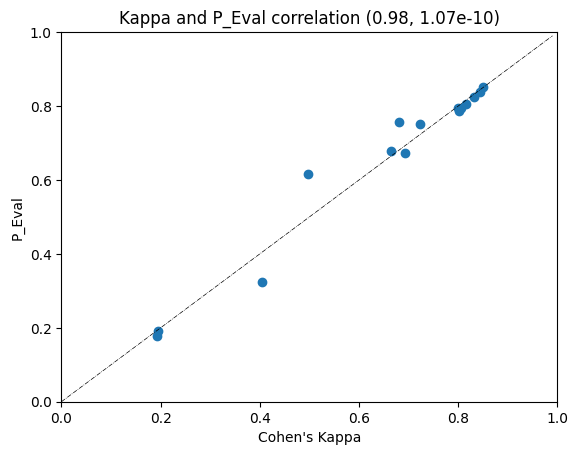
\includegraphics[width=\linewidth]{figures/eval-quality-kappa-correlation.png}
  \caption{Pearson's correlation coefficient between $\kappa$ and $P_e$ for \judgemodels.}
  \label{fig:k-p-corr}
\end{minipage}
\end{figure}


 

To estimate the inherent biases that might be present in the judge models, we present a simple hypothesis: For a given judge model and a given benchmark, the judge model correctly understands the task given to it and thus returns the correct evaluation with probability $P_e$. In the cases where the judge is not able to correctly understand the task, it randomly gives an evaluation of \texttt{true} with probability $P_+$, and an evaluation of \texttt{false} with the remaining probability of $1-P_+$.

The estimated probabilities using this method, with human evaluation as the reference, are shown in \cref{tab:pvals}. See Appendix XYZ for more details. We observe that the estimated evaluation probability $P_e$ is highly correlated to the Cohen's Kappa score of the judges, with a Person correlation coefficient of $0.98$, as shown in Fig. \cref{fig:k-p-corr}.

We observe that $P_+$ for most models is significantly higher than $0.5$, indicating a tendency of the judge models to evaluate a response as correct when they are not able to completely understand the prompt. 
% These biases are also observed in Section \cref{subsec:judge-ability}.

 

\section {Conclusion}

In summary, our research reveals significant misalignment between Judge LLM evaluations and human assessments, with no consistent patterns in final scores or rankings even when evaluations align. But, our study also demonstrates that lexical matching strategies, such as "contains match," outperform half of the Judge LLMs while preserving the accuracy of exam taker rankings as the best Judge model. Notably, GPT-4 emerges as the most consistent LLM across all metrics, albeit at a higher cost. However, a more cost-effective alternative could be utilizing LLama 3 70B as a Judge. Furthermore, we observe that smaller models tend to be more lenient, whereas larger models consistently yield superior results as Judge LLMs. 
We also find that Judge LLMs are highly sensitive to prompt variations, with performance declining with overly complex or ambiguous instructions. Furthermore, our comparison highlights the consistent underperformance of fine-tuned models compared to pre-trained ones in objective assessments. These findings underscore the need for refinement in automatic grading system and use of Judge LLMs.



% In conclusion, we report that evaluations from different judges align poorly with human judgement. Judge LLMs do not exhibit any signs of systematic biases that may help us make an argument to use them. We also 

% \kc{Basically summarize here what are the answers that we found for the research questions that we put forward in the Experiments section. All answers should directly follow form the results of the experiments we performed.}


% textbf{1)} How well do the evaluations from different judges align with human evaluations? \textbf{2)} How is a alignment of evaluations related to the alignment of the final scores given by the judges? \textbf{3)} How similar are the rankings of evaluation models generated by the judge models compared to the rankings by humans? \textbf{4)} How sensitive are the judge models to the specific prompt provided to them to give a judgement? \textbf{5)} What are the similarities and differences in the mistakes made by different judges?

% \subsection{Future Work}
% These baseline results are a lot different from the previous run I did, with the difference being a slight change in the template (delimiting the questions, answers and references with “```” ), and skipping high ref count questions (although I don’t think the second change would make a difference). So that shows that the exact template used can be a big factor in the evaluations, and even GPT-4 is susceptible to small changes in the template.

% \begin{ack}
% Use unnumbered first level headings for the acknowledgments. All acknowledgments
% go at the end of the paper before the list of references. Moreover, you are required to declare
% funding (financial activities supporting the submitted work) and competing interests (related financial activities outside the submitted work).
% More information about this disclosure can be found at: \url{https://neurips.cc/Conferences/2023/PaperInformation/FundingDisclosure}.


% Do {\bf not} include this section in the anonymized submission, only in the final paper. You can use the \texttt{ack} environment provided in the style file to autmoatically hide this section in the anonymized submission.
% \end{ack}



% \section{Supplementary Material}

% Authors may wish to optionally include extra information (complete proofs, additional experiments and plots) in the appendix. All such materials should be part of the supplemental material (submitted separately) and should NOT be included in the main submission.

%%%%%%%%%%%%%%%%%%%%%%%%%%%%%%%%%%%%%%%%%%%%%%%%%%%%%%%%%%%%
\bibliographystyle{acl_natbib}
\bibliography{bibliography}

\appendix
\renewcommand{\thesection}{\Alph{section}}

\section{Appendix}
\label{sec:Appendix}
% \kc{Should probably use actual examples instead of the generic templates.}

\subsection{Metrics for \judgemodels}
\label{app:metrics}

While the metric for evaluation of \evaluatormodels is the score assigned to them by \judgemodels, with higher score being better, the evaluation of a \judgemodel is based on how close the evaluations of the judge are to the ground-truth evaluations. In the absence of a ground-truth evaluation, the alignment of the evaluations from the \judgemodel can be measured against human judgements to evaluate the quality of evaluations from the \judgemodels. There are two common metrics used to quantify the agreement of evaluations between two annotators -- alignment ratio 
%\kc{better name?} 
and Cohen's kappa coefficient. We focus on the case of binary annotation, where each evaluation is one of two possible values (e.g., \texttt{correct} or \texttt{incorrect}). In this case, if one of the annotators is taken to be the reference, then the annotations of the other annotator can be categorized as true positives, false positives, true negatives, and false negatives, with the total number of each of them in a benchmark being represented by $T_P, F_P, T_N,$ and $F_N$ respectively.

\textbf{Alignment ratio} is simply the ratio of the numbers of times two annotators agree with each other relative to the total number of annotations. This ratio can have values between $0$ and $1$. For the binary case, the alignment ratio $\rho$ 
%\kc{what symbol to use?} 
is given as

\begin{equation}
    \rho = \frac{T_P + T_N}{T_P + F_P + T_N + F_N}.
\end{equation}

\textbf{Cohen's kappa coefficient}, or Cohen's kappa for short \citep{cohen1960kappa}, measures the alignment of two annotators while also taking into account the possibility of agreement by pure chance. This coefficient can have values between $-1$ and $1$, but is usually above $0$ in most real-world situations. The value of Cohen's kappa is given as

\begin{align}
    \kappa &= \frac{p_o - p_e}{1 - p_e} = \frac{2(T_PT_N - F_PF_N)}{(T_P+F_P)(T_N+F_P) + (T_P+F_N)(T_N+F_N)}.
\end{align}

This coefficient is considered to be a more robust measure of inter-annotator alignment, but also less interpretable in terms of what a particular value of $\kappa$ means. Generally, values of $\kappa$ in ranges $[0, 0.2)$, $[0.2, 0.4)$, $[0.4, 0.6)$, $[0.6, 0.8)$, and $[0.8, 1)$ are considered to indicate no alignment, slight alignment, moderate alignment, substantial alignment, and near-perfect alignment respectively, with $\kappa=1$ indicating perfect alignment. 


\subsection{Model Evaluation Prompt templates}\label{app:prompt-templates}

Here are the templates we use for the base and chat \evaluatormodels on the TriviaQA dataset

\begin{figure}[h]
    \centering
    \centering
    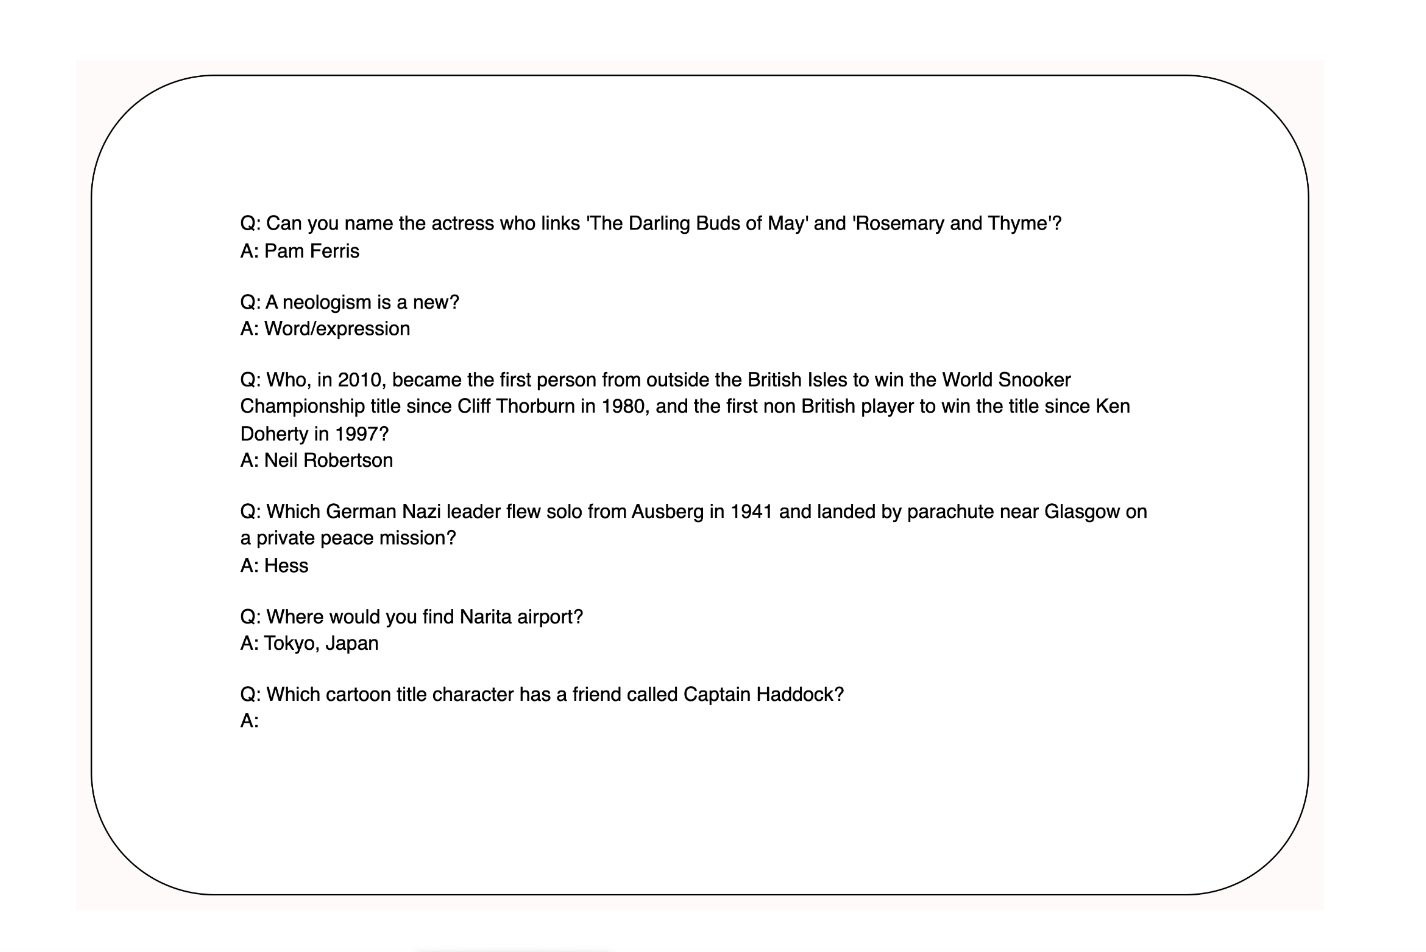
\includegraphics[width=\linewidth]{figures/Base_prompt_template.png}
    \caption{Prompt template for base models}
    \label{app:template_pretrained}
\end{figure}


\begin{figure}[H]
    \centering
    \centering
    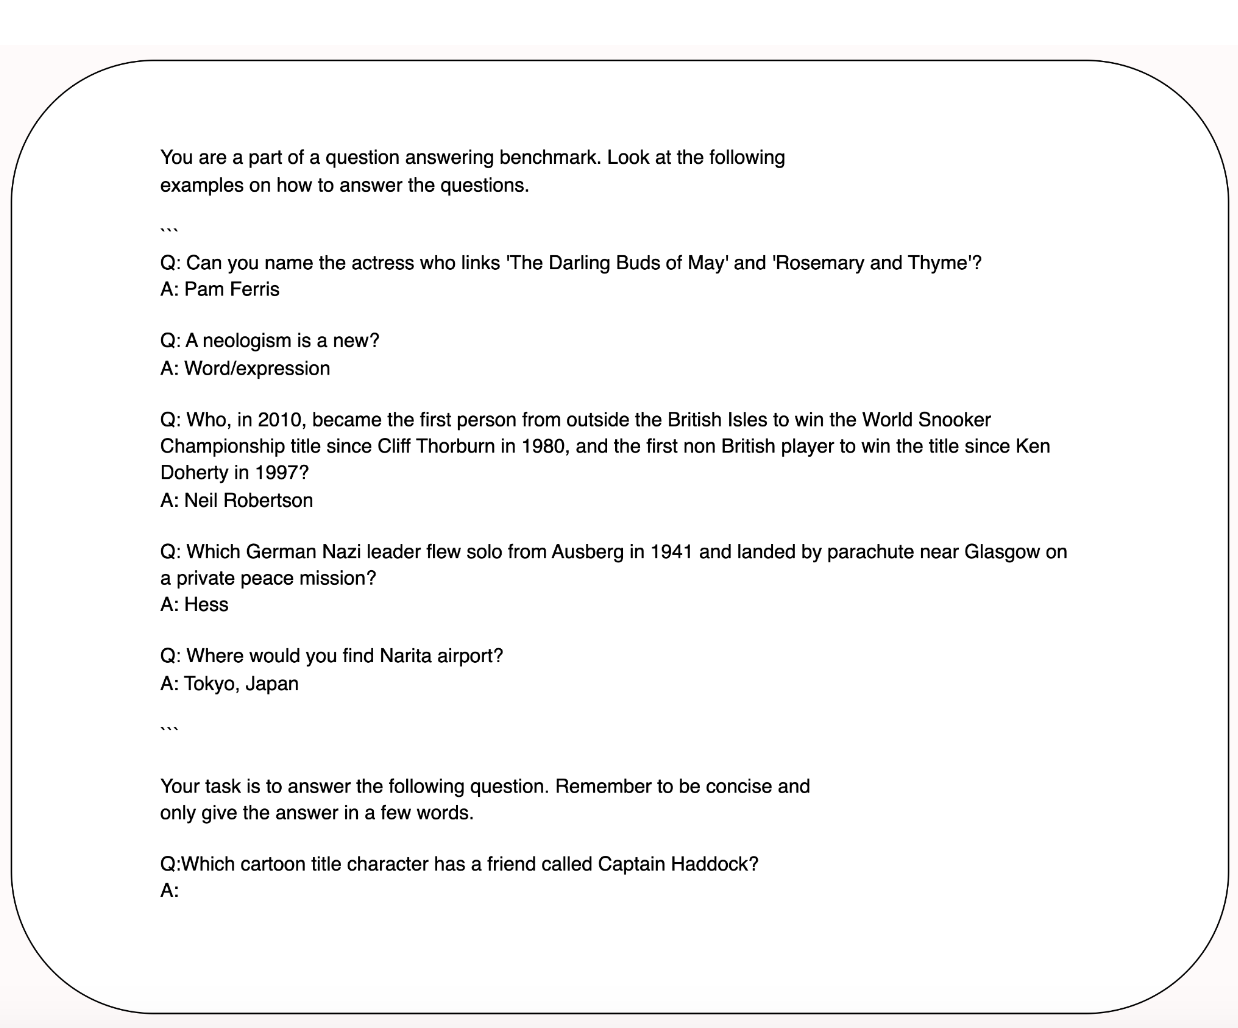
\includegraphics[width=\linewidth]{figures/Chat_prompt_template.png}
    \caption{Prompt template for Chat models}
    \label{app:template_finetuned}
\end{figure}


\subsection{Choice of Judge LLMs}
\label{app:judgeLLM_details}

To evaluate the efficacy of Judge LLMs of different sizes, we employ Mistral 7B \citep{jiang2023mistral}, Llama 2 models with 7B, 13B, and 70B parameters \citep{touvron2023llama}, and Llama 3 models with 8B and 70B parameters \citep{meta2024llama3}. Additionally, we include the Gemma 2B model \citep{gemma2024gemma} to assess the performance of smaller LLMs as judges. For comprehensive analysis, we also consider JudgeLM \citep{judgelm}, a model specifically fine-tuned for judge tasks, and GPT-4 \citep{openai2024gpt4}, a state-of-the-art large language model known for its close-to-human judgment performance, advanced language understanding, robust reasoning abilities, and versatility in processing diverse information.

\subsection{Judge LLM Prompt templates}\label{app:judge-prompt-template}

Prompt template for the \judgemodels

\begin{figure}[H]
    \centering
    \centering
    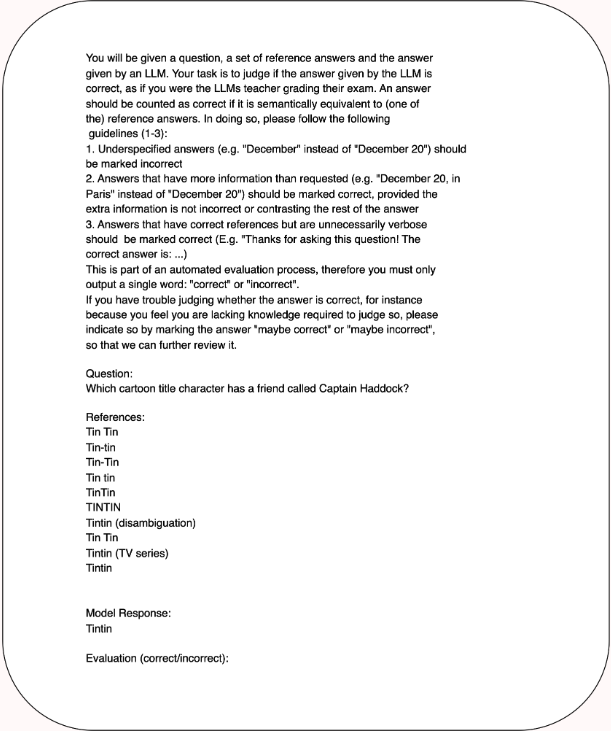
\includegraphics[width=\linewidth]{figures/Judge_Template.png}
    \caption{Prompt template for the \judgemodels}
    \label{app:judgeLLMs:prompts}
\end{figure}

\subsection{Human Annotation Guidelines}
\label{app:human_annotation_guidelines}
The guidelines are as follows -

You will be given a question, a set of reference answers and the answer given by an LLM. Your task is to judge if the answer given by the LLM is correct, as if you were the LLMs teacher grading their exam. An answer should be counted as correct if it is semantically equivalent to (one of the) reference answers. In doing so, please follow the following guidelines:
\begin{itemize}
    \item Underspecified answers (e.g. "December" instead of "December 20") should be marked \textit{incorrect}.
    \item Answers that have more information than requested (e.g. "December 20, in Paris" instead of "December 20") should be marked correct, provided the extra information is not incorrect or contrasting the rest of the answer.
    \item Answers with unnecessary verbosity but correct answers should be marked correct (E.g. ``Thanks for asking this question! The correct answer is: ...").
\end{itemize}
If you have trouble judging whether the answer is correct, for instance because you feel you are lacking knowledge required to judge so, please indicate so by marking the answer "maybe correct" or ``maybe incorrect", so that we can further review it.
\newpage
\subsection{Judge Score Models}
\textcolor{red}{Table Stale}
{\small
\setlength{\tabcolsep}{4pt} % Reduce padding between columns
\renewcommand{\arraystretch}{1.2} % Adjust the padding
\begin{longtable}{|p{1.5cm}|p{1.1cm}|p{1.1cm}|p{1.1cm}|p{1.1cm}|p{1.1cm}|p{1.1cm}|p{1.1cm}|p{1.1cm}|p{1.1cm}|p{1.1cm}|}
\hline
\multicolumn{2}{|c|}{\multirow{2}{*}{}} & \multicolumn{9}{|c|}{\textbf{Evaluator Models}} \\ \cline{3-11}
\multicolumn{2}{|c|}{\multirow{2}{*}{}} & \multicolumn{6}{c|}{Llama 2} & \multicolumn{2}{c|}{Mistral} & \multicolumn{1}{c|}{GPT-4} \\ \cline{3-11}
\multicolumn{2}{|c|}{} & \multicolumn{3}{c|}{Base} & \multicolumn{3}{c|}{Chat} & \multicolumn{1}{c|}{Base} & \multicolumn{1}{c|}{Instruct} &  \\ \hline
\multicolumn{2}{|c|}{\textbf{Judge Models}} & \multicolumn{1}{c|}{7B} & \multicolumn{1}{c|}{13B} & \multicolumn{1}{c|}{70B} & \multicolumn{1}{c|}{7B} & \multicolumn{1}{c|}{13B} & \multicolumn{1}{c|}{70B} & \multicolumn{2}{c|}{7B} &\\ \hline
\multicolumn{2}{|c|}{Exact Match} & 44.8 & 54.0 & 65 & 24 & 0.25 & 36.25 & 59 & 20.25 & 58  \\ \hline
\multicolumn{2}{|c|}{Human Eval} & 63.5 & 73.25 & 82.75 & 56 & 56.75 & 72.75 & 72 & 61.25 & 92  \\  \hline
\multicolumn{2}{|c|}{Contains Match} & 49.5 & 58.2 & 68.2 & 35.18 & 46.25 & 59.5 &  & 44.0 & 0 \\ \hline
\multicolumn{2}{|c|}{Gemma 2B FT}  & 49.25 & 59.5 & 69.2 & 68 & 44.25 & 75.25 & 73 & 79.5 & 92 \\ \hline
\multicolumn{2}{|c|}{JudgeLM}  & 57 & 65.8 & 76 & 0 & 0 & 0 & 0 & 0 & 0 \\   \hline
\multicolumn{2}{|c|}{Llama 2 7B Chat}  & 59.8 & 68.2 & 78.0 & 58 & 64.5 & 71 & 68 & 61.75 & 87 \\   \hline
\multicolumn{2}{|c|}{Llama 2 13B Chat}  & 59.0 & 69.75 & 78.3 & 46 & 32.25 & 60.75 & 57 & 52.5 & 73  \\ \hline
\multicolumn{2}{|c|}{Llama 2 70B Chat}  & 68.75 & 77.75 & 88.25 & 64.0 & 74.0 & 78.25 & 77.0 & 69.5 & 0 \\ \hline
\multicolumn{2}{|c|}{Mistral 7B Instruct}  & 68.75 & 76.5 & 87 & 65 & 70.5 & 78 & 74 & 69.25 & 93  \\ \hline
\multicolumn{2}{|c|}{GPT-4} & 65.0 & 74.25 & 85.0 & 0 & 0 & 0 & 0 & 0 & 0 \\ \hline
\multicolumn{2}{|c|}{Llama 3 8B Instruct} & 38.0 & 77.5 & 87.0 & 65 & 75.0 & 78.5 & 75 & 66.0 & 92 \\ \hline
\multicolumn{2}{|c|}{Llama 3 70B Instruct} & 68.3 & 75.25 & 87.25 & 0 & 68.5 & 78.25 & 0 & 65.0 & 0 \\ \hline
\caption{Evaluation Scores from Judge LLMs} % Add a caption (optional)
\label{tab:eval-scores} % Add a label for referencing (optional)
\end{longtable}
}

\subsection{Too Much Info Confuses the LLM}
\label{app:TMI}

\definecolor{myorange}{rgb}{1,0.6,0.2}
\definecolor{lightorange}{rgb}{1,0.9,0.8}

\tcbset{
  outerbox/.style={
    colback=white,
    colframe=black,
    fonttitle=\bfseries,
    boxrule=0.25mm,
    sharp corners,
    rounded corners,
  }
}


%%%%%%%%%%%%%%%%%%%%%%%%%%%%%%%%%%%%%%%%%
%Without Guidelines v1

\mytcolorbox{Without Guidelines v1}{Review the question and examine the references provided, then evaluate the model's response. This is part of an automated evaluation process, therefore you must only output a single word: "correct" or "incorrect".
}{\textbf{Question:} \\
Which Australian did Roger Federer defeat to win his first Wimbledon Men’s Singles title in 2003? \\
\\
\textbf{References:} \\
MARK PHILIPPOUSSIS \\
MARK PHILIPPOUSSIS \\
\\
\textbf{Model Response:} \\
Mark Philippoussis\\
\\
\textbf{Evaluation (correct/incorrect):}
}

%%%%%%%%%%%%%%%%%%%%%%%%%%%%%%%%%%%%
%Without Guidelines v2

\mytcolorbox{Without Guidelines v2}{Your task is to look at the following question, and based on the references provided, determine if the model's response is correct or incorrect. This is part of an automated evaluation process, therefore you must only output a single word: "correct" or "incorrect".
}{\textbf{Question:} \\
Which Australian did Roger Federer defeat to win his first Wimbledon Men’s Singles title in 2003? \\
\\
\textbf{References:} \\
MARK PHILIPPOUSSIS \\
MARK PHILIPPOUSSIS \\
\\
\textbf{Model Response:} \\
Mark Philippoussis \\
\\
\textbf{Evaluation (correct/incorrect):}
}

%%%%%%%%%%%%%%%%%%%%%%%%%%%%%%%%%%%%
%Error codes without Guidelines

\mytcolorbox{Error codes without Guidelines}{Review the Question and Examine the Reference: Carefully read and understand the question. Carefully read each of the reference provided for the question:\\
Consider the following error categories that could lead to an incorrect response:\\
1. Incorrect Entity (Wrong answer)\\
2. Too many Entities (Extra responses beyond the correct answers)\\
3. Underspecification (Incomplete answer)\\
4. Overspecification (Correct answer but with additional incorrect information)\\
5. Answers not in response\\
This is part of an automated evaluation process, therefore you must only
output a single word: "correct" or "incorrect".}{\textbf{Question:} \\
Which Australian did Roger Federer defeat to win his first Wimbledon Men’s Singles title in 2003? \\
\\
\textbf{References:} \\
MARK PHILIPPOUSSIS \\
MARK PHILIPPOUSSIS \\
\\
\textbf{Model Response:} \\
Mark Philippoussis \\
\\
\textbf{Evaluation (correct/incorrect):}
\label{app:error_codes_without_guidelines}
}

%%%%%%%%%%%%%%%%%%%%%%%%%%%%%%%%%%%%%%%%%%%%%%
%With Guidelines but no examples


\mytcolorbox{With Guidelines but no examples}{Review the Question and Examine the Reference: Carefully read and understand the question. Carefully read each of the reference provided for the question:\\
Evaluate the LLM Response based on guidelines (1-4):\\
1. Given the model response, only consider the part(s) of the response
answering the question, and ignore any extra text.\\
2. When evaluating the language model's answer, evaluate True if it matches
with at least one of the provided references otherwise False.\\
3. An answer and reference pair is considered a match if they are
semantically equivalent given the context of the question. This
determination should not require world knowledge from the human, and if it
does, consider it not a match. The answer must contain all the information
of the reference for it to be considered a match.\\
4. Considering there might be multiple correct answers, each answer must
match with at least one reference for the response to be considered correct
overall.\\
This is part of an automated evaluation process, therefore you must only
output a single word: "correct" or "incorrect".}{\textbf{Question:} \\
Which Australian did Roger Federer defeat to win his first Wimbledon Men’s Singles title in 2003? \\
\\
\textbf{References:} \\
MARK PHILIPPOUSSIS \\
MARK PHILIPPOUSSIS \\
\\
\textbf{Model Response:} \\
Mark Philippoussis \\
\\
\textbf{Evaluation (correct/incorrect):}
}

%%%%%%%%%%%%%%%%%%%%%%%%%%%%%%%%%%%%%%%%%%%%%%
%With Guidelines but no examples

\mytcolorbox{With Guidelines and examples}{You will be given a question, a set of reference answers and the answer given by an LLM. Your task is to judge if the answer given by the LLM is correct, as if you were the LLMs teacher grading their exam. An answer should be counted as correct if it is semantically equivalent to (one of the) reference answers. In doing so, please follow the following guidelines (1-3):\\
1. Underspecified answers (e.g. "December" instead of "December 20") should be marked incorrect \\
2. Answers that have more information than requested (e.g. "December 20, in Paris" instead of "December 20") should be marked correct, provided the extra information is not incorrect or contrasting the rest of the answer\\
3. Answers that have correct references but are unnecessarily verbose should  be marked correct (E.g. "Thanks for asking this question! The correct answer is: ...)\\
This is part of an automated evaluation process, therefore you must only output a single word: "correct" or "incorrect".\\
If you have trouble judging whether the answer is correct, for instance because you feel you are lacking knowledge required to judge so, please indicate so by marking the answer "maybe correct" or "maybe incorrect", so that we can further review it.}{\textbf{Question:} \\
Which Australian did Roger Federer defeat to win his first Wimbledon Men’s Singles title in 2003? \\
\\
\textbf{References:} \\
MARK PHILIPPOUSSIS \\
MARK PHILIPPOUSSIS \\
\\
\textbf{Model Response:} \\
Mark Philippoussis \\
\\
\textbf{Evaluation (correct/incorrect):}
}

\subsection{\Judgemodels are sensitive to reference order}
\dieuwke{Mention that this matches the position bias found by the llm-as-a-judge folks.}
In a follow-up experiment, we investigate the judges' sensitivity to the order in which the references are provided.
In this experiment, we provide the same prompt, question and model response, but shuffle the references, and we measure how consistent the \judgemodel's assessments are.
\dieuwke{Give formula of how we compute it.}
In \cref{table:reference_consistency}, we can that there is some variation in scores for different permutations of the references. 
This variation of score primarily comes down to the sensitivity of the Judge LLM to the order of references and its instruction following ability.
When the answer given my the exam-taker model matches any of the top references as opposed to the bottom listed, the \judgemodel prefers it and evaluates it as right. 
% Additionally another factor that makes a judge LLM a good judge is consistency.

Generally, the bigger judge models are more consistent, and are lesser sensitive to the reference order. 
The smaller order fail to capture all the information in the prompt, and sometimes judges a right answer as wrong, using their own knowledge for the judgement rather than going by the references. 

\begin{table}[h]
\centering
\vspace{0.5em} % Adjust the spacing here
\begin{tabular}{|c|c|c|c|c|c|c|c|c|}
\hline
& Exact-match & Llama2 7B & Llama2 13B & Llama2 70B & Mistral 7B & GPT 4T \\
\hline
Default & 42.00 & 49.50 & 52.50 & 62.00 & 61.50 & 57.25\\
\hline
Shuffled & 42.00 & 48.50 & 54.25 & 61.75 & 61.75 & 57.75\\
\hline
\end{tabular}
\vspace{1em} % Adjust the spacing between caption and table
\caption{Judgement Scores for different ordering of the references given during judging for Llama-7B Base as the Exam-taker model}\label{table:reference_consistency}
\end{table}

\subsection{Judge Rank Correlation Supplements}
\label{app:correlationcoefftable}
Below is the table of Spearman's rank correlation coefficient ($\rho$) with Human Judgement. $\rho$ > 0.7 is considered well aligned. 

\begin{table}[htbp]
    \centering
    \caption{Spearman Rank Correlation Coefficient $\rho$}
    \begin{tabular}{lc}
        \toprule
        Judges & $\rho$ \\
        \midrule
        Contains & 0.983 \\
        JudgeLM-7B & 0.983 \\
        GPT-4 & 0.933 \\
        Llama3-70B & 0.933 \\
        Mistral-7B & 0.917 \\
        Llama-13B & 0.817 \\
        EM & 0.783 \\
        Llama3-8B & 0.767 \\
        Llama-70B & 0.750 \\
        Llama-7B & 0.383 \\
        Gemma-2B & 0.208 \\
        \bottomrule
    \end{tabular}
    \label{tab:judges_rho_reversed}
\end{table}

\subsection{Base vs chat analysis supplementary}
\label{app:BaseVsChatSupp}

\label{app:correlationcoefftable}
\begin{figure}[H]
    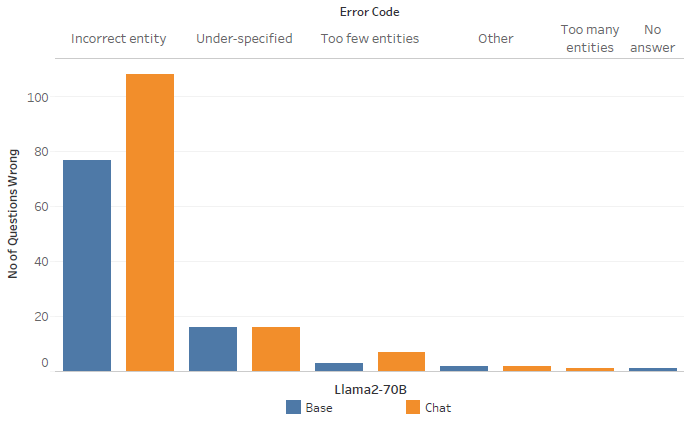
\includegraphics[width=\linewidth]{figures/Error_Codes_BarPlot.png}
    \caption{}
    \label{fig:comparisonBarplot}
    \caption{Incorrect questions count by error codes for \eval{Llama2 70B} Base vs Chat models}
     \label{fig:comparisonBarplot}
\end{figure}

\cref{fig:comparisonBarplot} shows that the \eval{Llama2 70B} Chat model answers a higher number of questions as 'incorrect entity' than the corresponding base model. Furthermore, the chat model provides too few entities in more responses than the base model, which also classifies as knowledge unlearning, since it cannot provide all the entities required for it to be correct.

\begin{figure}[h]
\centering
    \centering
    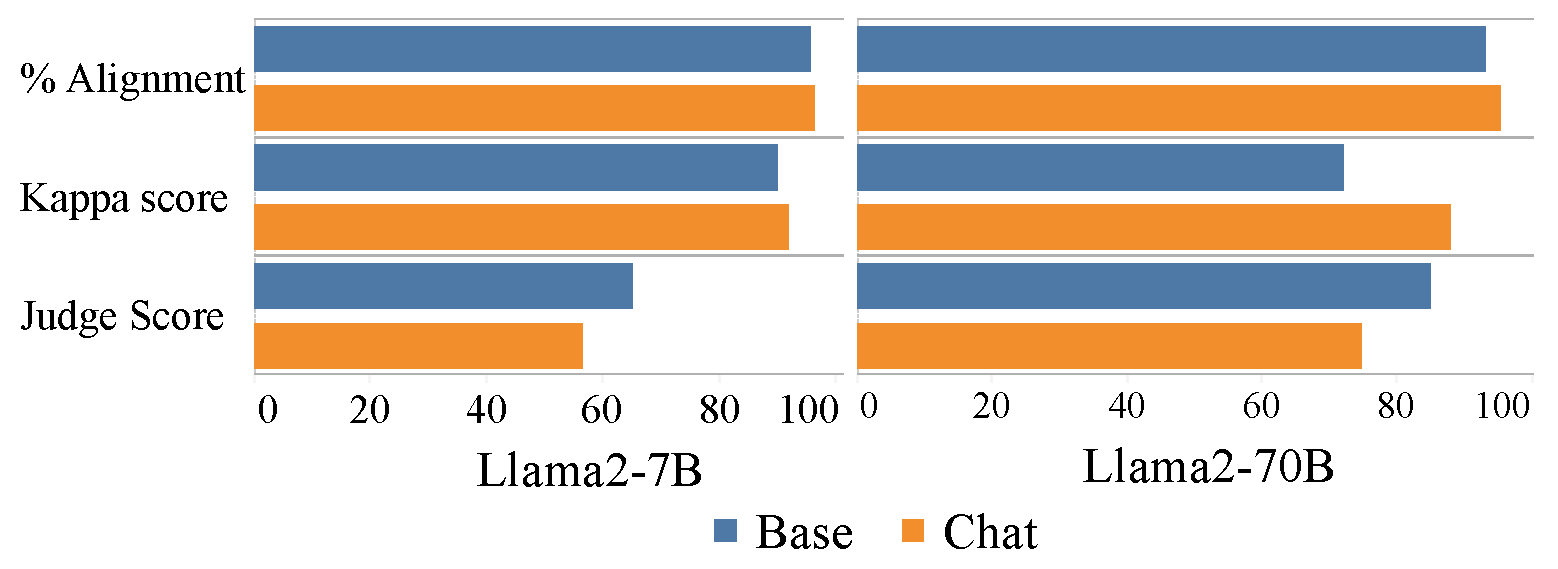
\includegraphics[width=\textwidth]{figures/BasevsChat.pdf}
    \caption{Evalaution Metrics for LLama2 7B and 70B Base and Chat pairs}
    \label{fig:BasevsChat}
\end{figure}


\definecolor{darkgreen}{rgb}{0.0, 0.5, 0.0}

\begin{table}[ht]
\centering
\begin{tabular}{|>{\raggedright\arraybackslash}m{2.5cm}|>{\raggedright\arraybackslash}m{10cm}|}
\hline
\multicolumn{2}{|c|}{\textbf{Question:}} \\
\multicolumn{2}{|c|}{Which British artist's works include 'The First Real Target'?} \\
\hline
\textbf{References} & \rule{0pt}{3ex}Peter Blake, Peter Balke, Sir Peter Blake\rule[-1ex]{0pt}{1ex} \\
\hline
\textbf{LLama-2 70B Base} & \rule{0pt}{3ex}\textcolor{darkgreen}{Peter Blake}\rule[-1ex]{0pt}{1ex} \\
\hline
\textbf{LLama-2 70B Chat} & \rule{0pt}{3ex}\textcolor{red}{Patrick Caulfield}\rule[-1ex]{0pt}{1ex} \\
\hline
\textbf{Mistral 7B Base} & \rule{0pt}{3ex}\textcolor{red}{David Hockney}\rule[-1ex]{0pt}{1ex} \\
\hline
\textbf{Mistral 7B Chat} & \rule{0pt}{3ex}\textcolor{red}{Damien Hirst}\rule[-1ex]{0pt}{1ex} \\
\hline
\end{tabular}
\caption{Knowledge Unlearning Example 1}
\label{tab:KnowledgeUnlearningExample1}
\end{table}

\begin{table}[ht]
\centering
\begin{tabular}{|>{\raggedright\arraybackslash}m{2.5cm}|>{\raggedright\arraybackslash}m{10cm}|}
\hline
\multicolumn{2}{|c|}{\textbf{Question:}} \\
\multicolumn{2}{|c|}{Who was the first cricketer to score 10,000 test runs?} \\
\hline
\textbf{References} & \rule{0pt}{3ex}Sunil Gavaskar, Sunil Manohar Gavaskar, SM Gavaskar, Sunny gavaskar, Gavaskar\rule[-1ex]{0pt}{1ex} \\
\hline
\textbf{LLama-2 70B Base} & \rule{0pt}{3ex}\textcolor{darkgreen}{Sunil Gavaskar}\rule[-1ex]{0pt}{1ex} \\
\hline
\textbf{LLama-2 70B Chat} & \rule{0pt}{3ex}\textcolor{red}{Sachin Tendulkar}\rule[-1ex]{0pt}{1ex} \\
\hline
\textbf{Mistral 7B Base} & \rule{0pt}{3ex}\textcolor{red}{Sachin Tendulkar}\rule[-1ex]{0pt}{1ex} \\
\hline
\textbf{Mistral 7B Chat} & \rule{0pt}{3ex}\textcolor{red}{Sachin Tendulkar} was the first cricketer to score 10,000 runs in Test matches.\rule[-1ex]{0pt}{1ex} \\
\hline
\end{tabular}
\caption{Knowledge Unlearning Example 2}
\label{tab:KnowledgeUnlearningExample2}
\end{table}


\begin{table}[ht]
\centering
\begin{tabular}{|>{\raggedright\arraybackslash}p{2.5cm}|>{\raggedright\arraybackslash}p{10cm}|}
\hline
\multicolumn{2}{|c|}{\textbf{Question:}} \\
\multicolumn{2}{|c|}{\parbox{12cm}{'Uncle Harry's Coat' was the first garment produced by which famous jacket manufacturer, based in Simonside, Newcastle Upon Tyne?}} \\
\hline
\textbf{References} & \rule{0pt}{3ex}Barbour\rule[-1ex]{0pt}{1ex} \\
\hline
\textbf{LLama-2 70B Base} & \rule{0pt}{3ex}\textcolor{darkgreen}{Barbour}\rule[-1ex]{0pt}{1ex} \\
\hline
\textbf{LLama-2 70B Chat} & \rule{0pt}{3ex}\textcolor{darkgreen}{Barbour}\rule[-1ex]{0pt}{1ex} \\
\hline
\textbf{Mistral 7B Base} & \rule{0pt}{3ex}\textcolor{darkgreen}{Barbour}\rule[-1ex]{0pt}{1ex} \\
\hline
\textbf{Mistral 7B Chat} & \rule{0pt}{3ex}\textcolor{red}{Jack Walker \& Sons}\rule[-1ex]{0pt}{1ex} \\
\hline
\end{tabular}
\caption{Knowledge Unlearning Example 3}
\label{tab:KnowledgeUnlearningExample2}
\end{table}

% \section*{NeurIPS Paper Checklist}

%%% BEGIN INSTRUCTIONS %%%
The checklist is designed to encourage best practices for responsible machine learning research, addressing issues of reproducibility, transparency, research ethics, and societal impact. Do not remove the checklist: {\bf The papers not including the checklist will be desk rejected.} The checklist should follow the references and precede the (optional) supplemental material.  The checklist does NOT count towards the page limit. 

Please read the checklist guidelines carefully for information on how to answer these questions. For each question in the checklist:
\begin{itemize}
    \item You should answer \verb+\answerYes{}+, \verb+\answerNo{}+, or \verb+\answerNA{}+.
    \item \verb+\answerNA{}+ means either that the question is Not Applicable for that particular paper or the relevant information is Not Available.
    \item Please provide a short (1–2 sentence) justification right after your answer (even for NA). 
   % \item {\bf The papers not including the checklist will be desk rejected.}
\end{itemize}

{\bf The checklist answers are an integral part of your paper submission.} They are visible to the reviewers, area chairs, senior area chairs, and ethics reviewers. You will be asked to also include it (after eventual revisions) with the final version of your paper, and its final version will be published with the paper.

The reviewers of your paper will be asked to use the checklist as one of the factors in their evaluation. While "\verb+\answerYes{}+" is generally preferable to "\verb+\answerNo{}+", it is perfectly acceptable to answer "\verb+\answerNo{}+" provided a proper justification is given (e.g., "error bars are not reported because it would be too computationally expensive" or "we were unable to find the license for the dataset we used"). In general, answering "\verb+\answerNo{}+" or "\verb+\answerNA{}+" is not grounds for rejection. While the questions are phrased in a binary way, we acknowledge that the true answer is often more nuanced, so please just use your best judgment and write a justification to elaborate. All supporting evidence can appear either in the main paper or the supplemental material, provided in appendix. If you answer \verb+\answerYes{}+ to a question, in the justification please point to the section(s) where related material for the question can be found.

IMPORTANT, please:
\begin{itemize}
    \item {\bf Delete this instruction block, but keep the section heading ``NeurIPS paper checklist"},
    \item  {\bf Keep the checklist subsection headings, questions/answers and guidelines below.}
    \item {\bf Do not modify the questions and only use the provided macros for your answers}.
\end{itemize} 
 

%%% END INSTRUCTIONS %%%


\begin{enumerate}

\item {\bf Claims}
    \item[] Question: Do the main claims made in the abstract and introduction accurately reflect the paper's contributions and scope?
    \item[] Answer: \verb+\answerTODO{}+ % Replace by \answerYes{}, \answerNo{}, or \answerNA{}.
    \item[] Justification: \verb+\justificationTODO{}+
    \item[] Guidelines:
    \begin{itemize}
        \item The answer NA means that the abstract and introduction do not include the claims made in the paper.
        \item The abstract and/or introduction should clearly state the claims made, including the contributions made in the paper and important assumptions and limitations. A No or NA answer to this question will not be perceived well by the reviewers. 
        \item The claims made should match theoretical and experimental results, and reflect how much the results can be expected to generalize to other settings. 
        \item It is fine to include aspirational goals as motivation as long as it is clear that these goals are not attained by the paper. 
    \end{itemize}

\item {\bf Limitations}
    \item[] Question: Does the paper discuss the limitations of the work performed by the authors?
    \item[] Answer: \verb+\answerTODO{}+ % Replace by \answerYes{}, \answerNo{}, or \answerNA{}.
    \item[] Justification: \verb+\justificationTODO{}+
    \item[] Guidelines:
    \begin{itemize}
        \item The answer NA means that the paper has no limitation while the answer No means that the paper has limitations, but those are not discussed in the paper. 
        \item The authors are encouraged to create a separate "Limitations" section in their paper.
        \item The paper should point out any strong assumptions and how robust the results are to violations of these assumptions (e.g., independence assumptions, noiseless settings, model well-specification, asymptotic approximations only holding locally). The authors should reflect on how these assumptions might be violated in practice and what the implications would be.
        \item The authors should reflect on the scope of the claims made, e.g., if the approach was only tested on a few datasets or with a few runs. In general, empirical results often depend on implicit assumptions, which should be articulated.
        \item The authors should reflect on the factors that influence the performance of the approach. For example, a facial recognition algorithm may perform poorly when image resolution is low or images are taken in low lighting. Or a speech-to-text system might not be used reliably to provide closed captions for online lectures because it fails to handle technical jargon.
        \item The authors should discuss the computational efficiency of the proposed algorithms and how they scale with dataset size.
        \item If applicable, the authors should discuss possible limitations of their approach to address problems of privacy and fairness.
        \item While the authors might fear that complete honesty about limitations might be used by reviewers as grounds for rejection, a worse outcome might be that reviewers discover limitations that aren't acknowledged in the paper. The authors should use their best judgment and recognize that individual actions in favor of transparency play an important role in developing norms that preserve the integrity of the community. Reviewers will be specifically instructed to not penalize honesty concerning limitations.
    \end{itemize}

\item {\bf Theory Assumptions and Proofs}
    \item[] Question: For each theoretical result, does the paper provide the full set of assumptions and a complete (and correct) proof?
    \item[] Answer: \verb+\answerTODO{}+ % Replace by \answerYes{}, \answerNo{}, or \answerNA{}.
    \item[] Justification: \verb+\justificationTODO{}+
    \item[] Guidelines:
    \begin{itemize}
        \item The answer NA means that the paper does not include theoretical results. 
        \item All the theorems, formulas, and proofs in the paper should be numbered and cross-referenced.
        \item All assumptions should be clearly stated or referenced in the statement of any theorems.
        \item The proofs can either appear in the main paper or the supplemental material, but if they appear in the supplemental material, the authors are encouraged to provide a short proof sketch to provide intuition. 
        \item Inversely, any informal proof provided in the core of the paper should be complemented by formal proofs provided in appendix or supplemental material.
        \item Theorems and Lemmas that the proof relies upon should be properly referenced. 
    \end{itemize}

    \item {\bf Experimental Result Reproducibility}
    \item[] Question: Does the paper fully disclose all the information needed to reproduce the main experimental results of the paper to the extent that it affects the main claims and/or conclusions of the paper (regardless of whether the code and data are provided or not)?
    \item[] Answer: \answerYes{} % Replace by \answerYes{}, \answerNo{}, or \answerNA{}.
    \item[] Justification: The code for benchmarking the \evaluatormodels and evaluating them using the \judgemodels, as well as the configuration files containing names and version numbers of the models and benchmarks are all present in the GitHub repository as well as the attached supplementary data. For human evaluations, the exact guidelines used by human evaluators are provided in \cref{XYZ}.
    \item[] Guidelines:
    \begin{itemize}
        \item The answer NA means that the paper does not include experiments.
        \item If the paper includes experiments, a No answer to this question will not be perceived well by the reviewers: Making the paper reproducible is important, regardless of whether the code and data are provided or not.
        \item If the contribution is a dataset and/or model, the authors should describe the steps taken to make their results reproducible or verifiable. 
        \item Depending on the contribution, reproducibility can be accomplished in various ways. For example, if the contribution is a novel architecture, describing the architecture fully might suffice, or if the contribution is a specific model and empirical evaluation, it may be necessary to either make it possible for others to replicate the model with the same dataset, or provide access to the model. In general. releasing code and data is often one good way to accomplish this, but reproducibility can also be provided via detailed instructions for how to replicate the results, access to a hosted model (e.g., in the case of a large language model), releasing of a model checkpoint, or other means that are appropriate to the research performed.
        \item While NeurIPS does not require releasing code, the conference does require all submissions to provide some reasonable avenue for reproducibility, which may depend on the nature of the contribution. For example
        \begin{enumerate}
            \item If the contribution is primarily a new algorithm, the paper should make it clear how to reproduce that algorithm.
            \item If the contribution is primarily a new model architecture, the paper should describe the architecture clearly and fully.
            \item If the contribution is a new model (e.g., a large language model), then there should either be a way to access this model for reproducing the results or a way to reproduce the model (e.g., with an open-source dataset or instructions for how to construct the dataset).
            \item We recognize that reproducibility may be tricky in some cases, in which case authors are welcome to describe the particular way they provide for reproducibility. In the case of closed-source models, it may be that access to the model is limited in some way (e.g., to registered users), but it should be possible for other researchers to have some path to reproducing or verifying the results.
        \end{enumerate}
    \end{itemize}


\item {\bf Open access to data and code}
    \item[] Question: Does the paper provide open access to the data and code, with sufficient instructions to faithfully reproduce the main experimental results, as described in supplemental material?
    \item[] Answer: \answerYes{} % Replace by \answerYes{}, \answerNo{}, or \answerNA{}.
    \item[] Justification: The code for running all experiments in this work has been made available in the supplementary material and on GitHub, along with information of the names and versions of models and datasets used in the experiments. Specific instructions for running the experiments to reproduce the results in this work are also provided.
    \item[] Guidelines:
    \begin{itemize}
        \item The answer NA means that paper does not include experiments requiring code.
        \item Please see the NeurIPS code and data submission guidelines (\url{https://nips.cc/public/guides/CodeSubmissionPolicy}) for more details.
        \item While we encourage the release of code and data, we understand that this might not be possible, so “No” is an acceptable answer. Papers cannot be rejected simply for not including code, unless this is central to the contribution (e.g., for a new open-source benchmark).
        \item The instructions should contain the exact command and environment needed to run to reproduce the results. See the NeurIPS code and data submission guidelines (\url{https://nips.cc/public/guides/CodeSubmissionPolicy}) for more details.
        \item The authors should provide instructions on data access and preparation, including how to access the raw data, preprocessed data, intermediate data, and generated data, etc.
        \item The authors should provide scripts to reproduce all experimental results for the new proposed method and baselines. If only a subset of experiments are reproducible, they should state which ones are omitted from the script and why.
        \item At submission time, to preserve anonymity, the authors should release anonymized versions (if applicable).
        \item Providing as much information as possible in supplemental material (appended to the paper) is recommended, but including URLs to data and code is permitted.
    \end{itemize}


\item {\bf Experimental Setting/Details}
    \item[] Question: Does the paper specify all the training and test details (e.g., data splits, hyperparameters, how they were chosen, type of optimizer, etc.) necessary to understand the results?
    \item[] Answer: \answerYes{} % Replace by \answerYes{}, \answerNo{}, or \answerNA{}.
    \item[] Justification: All experimental details, including hyperparameters, model names and version, and seed values are provided in \cref{XYZ}.
    \item[] Guidelines:
    \begin{itemize}
        \item The answer NA means that the paper does not include experiments.
        \item The experimental setting should be presented in the core of the paper to a level of detail that is necessary to appreciate the results and make sense of them.
        \item The full details can be provided either with the code, in appendix, or as supplemental material.
    \end{itemize}

\item {\bf Experiment Statistical Significance}
    \item[] Question: Does the paper report error bars suitably and correctly defined or other appropriate information about the statistical significance of the experiments?
    \item[] Answer: \verb+\answerTODO{}+ % Replace by \answerYes{}, \answerNo{}, or \answerNA{}.
    \item[] Justification: \verb+\justificationTODO{}+
    \item[] Guidelines:
    \begin{itemize}
        \item The answer NA means that the paper does not include experiments.
        \item The authors should answer "Yes" if the results are accompanied by error bars, confidence intervals, or statistical significance tests, at least for the experiments that support the main claims of the paper.
        \item The factors of variability that the error bars are capturing should be clearly stated (for example, train/test split, initialization, random drawing of some parameter, or overall run with given experimental conditions).
        \item The method for calculating the error bars should be explained (closed form formula, call to a library function, bootstrap, etc.)
        \item The assumptions made should be given (e.g., Normally distributed errors).
        \item It should be clear whether the error bar is the standard deviation or the standard error of the mean.
        \item It is OK to report 1-sigma error bars, but one should state it. The authors should preferably report a 2-sigma error bar than state that they have a 96\% CI, if the hypothesis of Normality of errors is not verified.
        \item For asymmetric distributions, the authors should be careful not to show in tables or figures symmetric error bars that would yield results that are out of range (e.g. negative error rates).
        \item If error bars are reported in tables or plots, The authors should explain in the text how they were calculated and reference the corresponding figures or tables in the text.
    \end{itemize}

\item {\bf Experiments Compute Resources}
    \item[] Question: For each experiment, does the paper provide sufficient information on the computer resources (type of compute workers, memory, time of execution) needed to reproduce the experiments?
    \item[] Answer: \verb+\answerTODO{}+ % Replace by \answerYes{}, \answerNo{}, or \answerNA{}.
    \item[] Justification: \verb+\justificationTODO{}+
    \item[] Guidelines:
    \begin{itemize}
        \item The answer NA means that the paper does not include experiments.
        \item The paper should indicate the type of compute workers CPU or GPU, internal cluster, or cloud provider, including relevant memory and storage.
        \item The paper should provide the amount of compute required for each of the individual experimental runs as well as estimate the total compute. 
        \item The paper should disclose whether the full research project required more compute than the experiments reported in the paper (e.g., preliminary or failed experiments that didn't make it into the paper). 
    \end{itemize}
    
\item {\bf Code Of Ethics}
    \item[] Question: Does the research conducted in the paper conform, in every respect, with the NeurIPS Code of Ethics \url{https://neurips.cc/public/EthicsGuidelines}?
    \item[] Answer: \answerYes{} % Replace by \answerYes{}, \answerNo{}, or \answerNA{}.
    \item[] Justification: This work complies with NeurIPS Code of Ethics as well as all other applicable ethical and legal requirements. This work did not use the services of humans outside the research team itself, and all datasets and models used for experiments are publicly available (either freely or for a fee), and were used in compliance with their terms of service.
    \item[] Guidelines:
    \begin{itemize}
        \item The answer NA means that the authors have not reviewed the NeurIPS Code of Ethics.
        \item If the authors answer No, they should explain the special circumstances that require a deviation from the Code of Ethics.
        \item The authors should make sure to preserve anonymity (e.g., if there is a special consideration due to laws or regulations in their jurisdiction).
    \end{itemize}


\item {\bf Broader Impacts}
    \item[] Question: Does the paper discuss both potential positive societal impacts and negative societal impacts of the work performed?
    \item[] Answer: \verb+\answerTODO{}+ % Replace by \answerYes{}, \answerNo{}, or \answerNA{}.
    \item[] Justification: \verb+\justificationTODO{}+
    \item[] Guidelines:
    \begin{itemize}
        \item The answer NA means that there is no societal impact of the work performed.
        \item If the authors answer NA or No, they should explain why their work has no societal impact or why the paper does not address societal impact.
        \item Examples of negative societal impacts include potential malicious or unintended uses (e.g., disinformation, generating fake profiles, surveillance), fairness considerations (e.g., deployment of technologies that could make decisions that unfairly impact specific groups), privacy considerations, and security considerations.
        \item The conference expects that many papers will be foundational research and not tied to particular applications, let alone deployments. However, if there is a direct path to any negative applications, the authors should point it out. For example, it is legitimate to point out that an improvement in the quality of generative models could be used to generate deepfakes for disinformation. On the other hand, it is not needed to point out that a generic algorithm for optimizing neural networks could enable people to train models that generate Deepfakes faster.
        \item The authors should consider possible harms that could arise when the technology is being used as intended and functioning correctly, harms that could arise when the technology is being used as intended but gives incorrect results, and harms following from (intentional or unintentional) misuse of the technology.
        \item If there are negative societal impacts, the authors could also discuss possible mitigation strategies (e.g., gated release of models, providing defenses in addition to attacks, mechanisms for monitoring misuse, mechanisms to monitor how a system learns from feedback over time, improving the efficiency and accessibility of ML).
    \end{itemize}
    
\item {\bf Safeguards}
    \item[] Question: Does the paper describe safeguards that have been put in place for responsible release of data or models that have a high risk for misuse (e.g., pretrained language models, image generators, or scraped datasets)?
    \item[] Answer: \verb+\answerTODO{}+ % Replace by \answerYes{}, \answerNo{}, or \answerNA{}.
    \item[] Justification: \verb+\justificationTODO{}+
    \item[] Guidelines:
    \begin{itemize}
        \item The answer NA means that the paper poses no such risks.
        \item Released models that have a high risk for misuse or dual-use should be released with necessary safeguards to allow for controlled use of the model, for example by requiring that users adhere to usage guidelines or restrictions to access the model or implementing safety filters. 
        \item Datasets that have been scraped from the Internet could pose safety risks. The authors should describe how they avoided releasing unsafe images.
        \item We recognize that providing effective safeguards is challenging, and many papers do not require this, but we encourage authors to take this into account and make a best faith effort.
    \end{itemize}

\item {\bf Licenses for existing assets}
    \item[] Question: Are the creators or original owners of assets (e.g., code, data, models), used in the paper, properly credited and are the license and terms of use explicitly mentioned and properly respected?
    \item[] Answer: \verb+\answerTODO{}+ % Replace by \answerYes{}, \answerNo{}, or \answerNA{}.
    \item[] Justification: \verb+\justificationTODO{}+
    \item[] Guidelines:
    \begin{itemize}
        \item The answer NA means that the paper does not use existing assets.
        \item The authors should cite the original paper that produced the code package or dataset.
        \item The authors should state which version of the asset is used and, if possible, include a URL.
        \item The name of the license (e.g., CC-BY 4.0) should be included for each asset.
        \item For scraped data from a particular source (e.g., website), the copyright and terms of service of that source should be provided.
        \item If assets are released, the license, copyright information, and terms of use in the package should be provided. For popular datasets, \url{paperswithcode.com/datasets} has curated licenses for some datasets. Their licensing guide can help determine the license of a dataset.
        \item For existing datasets that are re-packaged, both the original license and the license of the derived asset (if it has changed) should be provided.
        \item If this information is not available online, the authors are encouraged to reach out to the asset's creators.
    \end{itemize}

\item {\bf New Assets}
    \item[] Question: Are new assets introduced in the paper well documented and is the documentation provided alongside the assets?
    \item[] Answer: \verb+\answerTODO{}+ % Replace by \answerYes{}, \answerNo{}, or \answerNA{}.
    \item[] Justification: \verb+\justificationTODO{}+
    \item[] Guidelines:
    \begin{itemize}
        \item The answer NA means that the paper does not release new assets.
        \item Researchers should communicate the details of the dataset/code/model as part of their submissions via structured templates. This includes details about training, license, limitations, etc. 
        \item The paper should discuss whether and how consent was obtained from people whose asset is used.
        \item At submission time, remember to anonymize your assets (if applicable). You can either create an anonymized URL or include an anonymized zip file.
    \end{itemize}

\item {\bf Crowdsourcing and Research with Human Subjects}
    \item[] Question: For crowdsourcing experiments and research with human subjects, does the paper include the full text of instructions given to participants and screenshots, if applicable, as well as details about compensation (if any)? 
    \item[] Answer: \verb+\answerTODO{}+ % Replace by \answerYes{}, \answerNo{}, or \answerNA{}.
    \item[] Justification: \verb+\justificationTODO{}+
    \item[] Guidelines:
    \begin{itemize}
        \item The answer NA means that the paper does not involve crowdsourcing nor research with human subjects.
        \item Including this information in the supplemental material is fine, but if the main contribution of the paper involves human subjects, then as much detail as possible should be included in the main paper. 
        \item According to the NeurIPS Code of Ethics, workers involved in data collection, curation, or other labor should be paid at least the minimum wage in the country of the data collector. 
    \end{itemize}

\item {\bf Institutional Review Board (IRB) Approvals or Equivalent for Research with Human Subjects}
    \item[] Question: Does the paper describe potential risks incurred by study participants, whether such risks were disclosed to the subjects, and whether Institutional Review Board (IRB) approvals (or an equivalent approval/review based on the requirements of your country or institution) were obtained?
    \item[] Answer: \answerNA{} % Replace by \answerYes{}, \answerNo{}, or \answerNA{}.
    \item[] Justification: This work does not involve any human subjects. All human annotations in the results were done by the authors themselves.
    \item[] Guidelines:
    \begin{itemize}
        \item The answer NA means that the paper does not involve crowdsourcing nor research with human subjects.
        \item Depending on the country in which research is conducted, IRB approval (or equivalent) may be required for any human subjects research. If you obtained IRB approval, you should clearly state this in the paper. 
        \item We recognize that the procedures for this may vary significantly between institutions and locations, and we expect authors to adhere to the NeurIPS Code of Ethics and the guidelines for their institution. 
        \item For initial submissions, do not include any information that would break anonymity (if applicable), such as the institution conducting the review.
    \end{itemize}

\end{enumerate}

\end{document}
